\chapter{Methodology}

This paper is based on the ideas of the AlphaZero framework applied to the game of Damath. Damath is a two-player board game combining the Filipino Checkers ``Dama'' and Mathematics. Each piece has a corresponding number and every white square on the board has a mathematical operation. The researchers used the same architecture as a vision transformer and implemented the AlphaZero framework to train this model. The process in the AlphaZero framework is a cycle of three stages. The process first generates data through self-play using the modified Monte-Carlo Tree Search algorithm of AlphaZero. Afterwards, the model is trained on the data generated from self-play. Finally, the current version of the model is evaluated by pitting it against the previous model through competition.  After this process is completed, the final model is pitted against previous models and an expert Damath player for analysis of the model's competence.

\section{State Representation}
% ADVISERwCOMMENT (DON'T DELETE): add an example of the matrix
The state of the game is encoded as a $32 \times 23$ matrix where each row in the matrix represents a white cell on the board and each column represents a feature as shown in Table \ref{tab:state-representation-damath}. 

% ADVISER COMMENT (DON'T DELETE): need to rewrite this sentence to make it clearer. what happened eo the columns of the matrix?

\begin{table}[H]
  \centering
  \begin{tabular}{lll}
    \hline 
    Column & Type    & Feature                                                  \\ \hline
    1         & Boolean & Current Player of the Game                               \\
    2-14      & Boolean & Value of the Piece on the Current Cell                   \\
    15        & Boolean & Dama Status of Piece on the Current Cell                 \\
    16        & Boolean & Owner of the Piece on the Current Cell                   \\
    17        & Float   & Relative Score of the Current Player of the Game         \\
    18        & Float   & Current Draw Count of the Game                           \\
    19-22     & Boolean & Board Operator on the Current Cell                       \\
    23        & Boolean & Multiple Capture Status of the Piece on the Current Cell \\ \hline
  \end{tabular}
  \caption{State Representation of Damath}
  \label{tab:state-representation-damath}
\end{table}

To understand this further, we provide the example state representation of a state with the 10 dama piece of the red player performing a multiple capture move as shown in Figure \ref{fig:example-state-representation} and the current red player having a relative score of 0.6.

\newcommand{\gz}{\textcolor{black!10}{0}}
\newcommand{\gs}{\textcolor{black!10}{0.6}}
\newcommand{\go}{\textcolor{black!10}{1}}
\newcommand{\rz}{\textcolor{red}{0}}
\newcommand{\rs}{\textcolor{red}{0.6}}
\newcommand{\ro}{\textcolor{red}{1}}
\setcounter{MaxMatrixCols}{23}

% ADVISER COMMENT (DON'T DELETE,2025-05-30): try to make the equation/image a bit larger. if necessary make this into an image instead of an equation. at the very least, make the image (example_state.png) larger

\begin{figure}[H]
    \begin{equation*} 
        \verb|Encode|\left(\begin{gathered}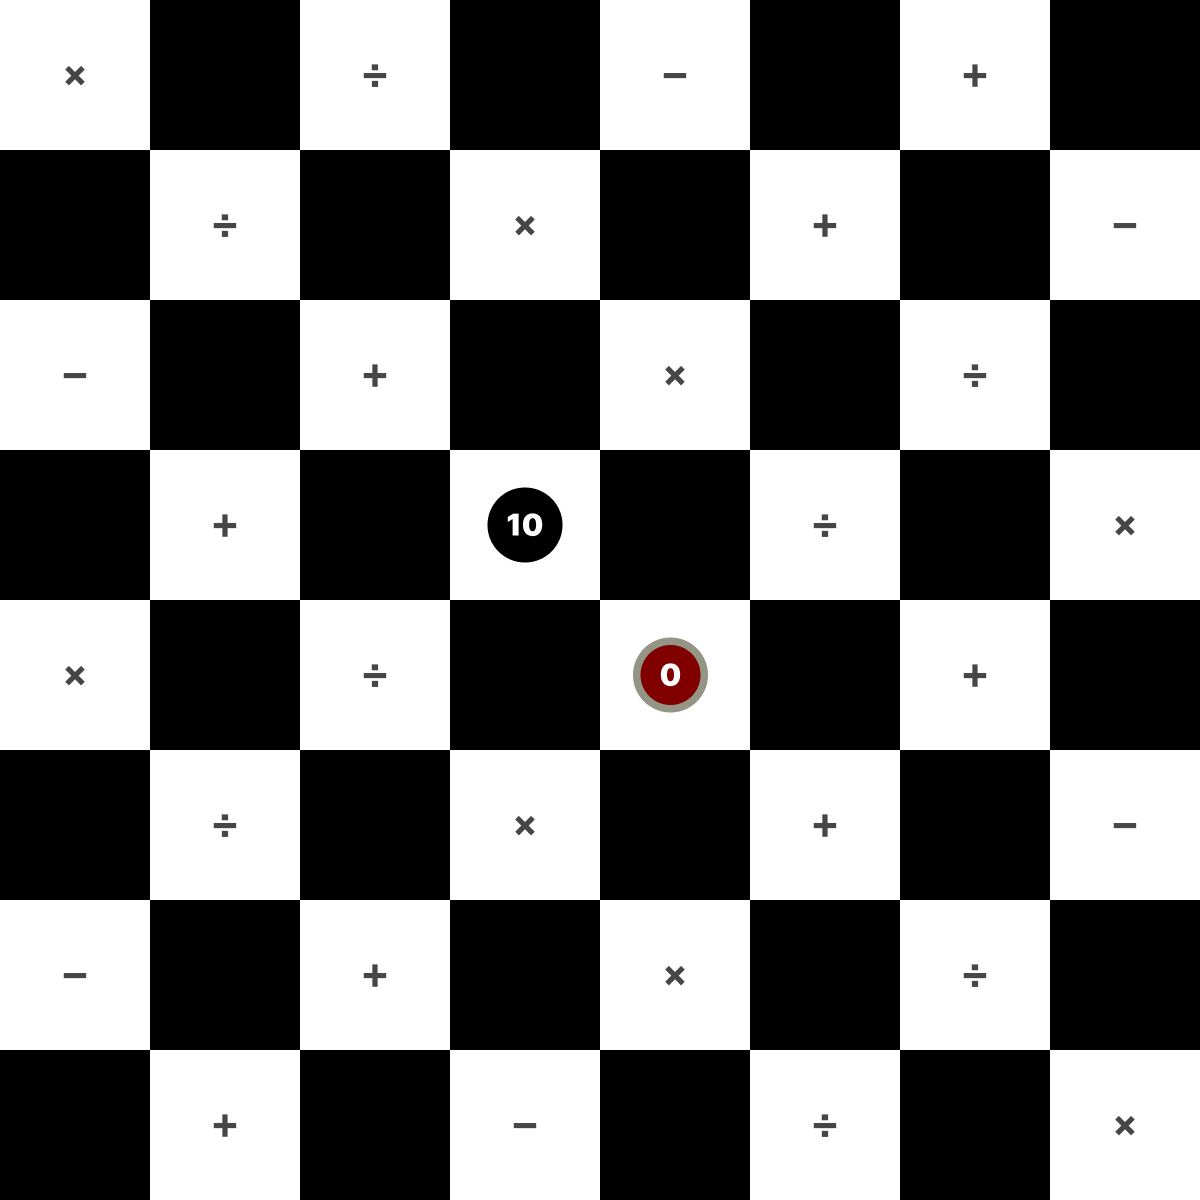
\includegraphics[width=0.4\linewidth]{images/example_state.png}\end{gathered}\right) = \resizebox{0.4\textwidth}{!}{$\begin{bmatrix}
            \gz & \gz & \gz & \gz & \gz & \gz & \gz & \gz & \gz & \gz & \gz & \gz & \gz & \gz & \gz & \textcolor{black!60}{0.6} & \gz & 1   & \gz & \gz & \gz & \gz \\
            \gz & \gz & \gz & \gz & \gz & \gz & \gz & \gz & \gz & \gz & \gz & \gz & \gz & \gz & \gz & \textcolor{black!60}{0.6} & \gz & \gz & 1   & \gz & \gz & \gz \\
            \gz & \gz & \gz & \gz & \gz & \gz & \gz & \gz & \gz & \gz & \gz & \gz & \gz & \gz & \gz & \textcolor{black!60}{0.6} & \gz & \gz & \gz & \gz & 1   & \gz \\
            \gz & \gz & \gz & \gz & \gz & \gz & \gz & \gz & \gz & \gz & \gz & \gz & \gz & \gz & \gz & \textcolor{black!60}{0.6} & \gz & \gz & \gz & 1   & \gz & \gz \\
            \gz & \gz & \gz & \gz & \gz & \gz & \gz & \gz & \gz & \gz & \gz & \gz & \gz & \gz & \gz & \textcolor{black!60}{0.6} & \gz & \gz & 1   & \gz & \gz & \gz \\
            \gz & \gz & \gz & \gz & \gz & \gz & \gz & \gz & \gz & \gz & \gz & \gz & \gz & \gz & \gz & \textcolor{black!60}{0.6} & \gz & 1   & \gz & \gz & \gz & \gz \\
            \gz & \gz & \gz & \gz & \gz & \gz & \gz & \gz & \gz & \gz & \gz & \gz & \gz & \gz & \gz & \textcolor{black!60}{0.6} & \gz & \gz & \gz & 1   & \gz & \gz \\
            \gz & \gz & \gz & \gz & \gz & \gz & \gz & \gz & \gz & \gz & \gz & \gz & \gz & \gz & \gz & \textcolor{black!60}{0.6} & \gz & \gz & \gz & \gz & 1   & \gz \\
            \gz & \gz & \gz & \gz & \gz & \gz & \gz & \gz & \gz & \gz & \gz & \gz & \gz & \gz & \gz & \textcolor{black!60}{0.6} & \gz & \gz & \gz & \gz & 1   & \gz \\
            \gz & \gz & \gz & \gz & \gz & \gz & \gz & \gz & \gz & \gz & \gz & \gz & \gz & \gz & \gz & \textcolor{black!60}{0.6} & \gz & \gz & \gz & 1   & \gz & \gz \\
            \gz & \gz & \gz & \gz & \gz & \gz & \gz & \gz & \gz & \gz & \gz & \gz & \gz & \gz & \gz & \textcolor{black!60}{0.6} & \gz & 1   & \gz & \gz & \gz & \gz \\
            \gz & \gz & \gz & \gz & \gz & \gz & \gz & \gz & \gz & \gz & \gz & \gz & \gz & \gz & \gz & \textcolor{black!60}{0.6} & \gz & \gz & 1   & \gz & \gz & \gz \\
            \gz & \gz & \gz & \gz & \gz & \gz & \gz & \gz & \gz & \gz & \gz & \gz & \gz & \gz & \gz & \textcolor{black!60}{0.6} & \gz & \gz & \gz & 1   & \gz & \gz \\
            \gz & \gz & \gz & \gz & \gz & \gz & \gz & \gz & \gz & \gz & \gz & \gz & \gz & \gz & \gz & \textcolor{black!60}{0.6} & \gz & \gz & \gz & \gz & 1   & \gz \\
            \gz & 1   & \gz & \gz & \gz & \gz & \gz & \gz & \gz & \gz & \gz & \gz & \gz & 1   & 1   & \textcolor{black!60}{0.6} & \gz & \gz & 1   & \gz & \gz & 1   \\
            \gz & \gz & \gz & \gz & \gz & \gz & \gz & \gz & \gz & \gz & \gz & \gz & \gz & \gz & \gz & \textcolor{black!60}{0.6} & \gz & 1   & \gz & \gz & \gz & \gz \\
            \gz & \gz & \gz & \gz & \gz & \gz & \gz & \gz & \gz & \gz & \gz & \gz & \gz & \gz & \gz & \textcolor{black!60}{0.6} & \gz & 1   & \gz & \gz & \gz & \gz \\
            \gz & \gz & \gz & \gz & \gz & \gz & \gz & \gz & \gz & \gz & \gz & 1   & \gz & \gz & \gz & \textcolor{black!60}{0.6} & \gz & \gz & 1   & \gz & \gz & \gz \\
            \gz & \gz & \gz & \gz & \gz & \gz & \gz & \gz & \gz & \gz & \gz & \gz & \gz & \gz & \gz & \textcolor{black!60}{0.6} & \gz & \gz & \gz & \gz & 1   & \gz \\
            \gz & \gz & \gz & \gz & \gz & \gz & \gz & \gz & \gz & \gz & \gz & \gz & \gz & \gz & \gz & \textcolor{black!60}{0.6} & \gz & \gz & \gz & 1   & \gz & \gz \\
            \gz & \gz & \gz & \gz & \gz & \gz & \gz & \gz & \gz & \gz & \gz & \gz & \gz & \gz & \gz & \textcolor{black!60}{0.6} & \gz & \gz & 1   & \gz & \gz & \gz \\
            \gz & \gz & \gz & \gz & \gz & \gz & \gz & \gz & \gz & \gz & \gz & \gz & \gz & \gz & \gz & \textcolor{black!60}{0.6} & \gz & 1   & \gz & \gz & \gz & \gz \\
            \gz & \gz & \gz & \gz & \gz & \gz & \gz & \gz & \gz & \gz & \gz & \gz & \gz & \gz & \gz & \textcolor{black!60}{0.6} & \gz & \gz & \gz & 1   & \gz & \gz \\
            \gz & \gz & \gz & \gz & \gz & \gz & \gz & \gz & \gz & \gz & \gz & \gz & \gz & \gz & \gz & \textcolor{black!60}{0.6} & \gz & \gz & \gz & \gz & 1   & \gz \\
            \gz & \gz & \gz & \gz & \gz & \gz & \gz & \gz & \gz & \gz & \gz & \gz & \gz & \gz & \gz & \textcolor{black!60}{0.6} & \gz & \gz & \gz & \gz & 1   & \gz \\
            \gz & \gz & \gz & \gz & \gz & \gz & \gz & \gz & \gz & \gz & \gz & \gz & \gz & \gz & \gz & \textcolor{black!60}{0.6} & \gz & \gz & \gz & 1   & \gz & \gz \\
            \gz & \gz & \gz & \gz & \gz & \gz & \gz & \gz & \gz & \gz & \gz & \gz & \gz & \gz & \gz & \textcolor{black!60}{0.6} & \gz & 1   & \gz & \gz & \gz & \gz \\
            \gz & \gz & \gz & \gz & \gz & \gz & \gz & \gz & \gz & \gz & \gz & \gz & \gz & \gz & \gz & \textcolor{black!60}{0.6} & \gz & \gz & 1   & \gz & \gz & \gz \\
            \gz & \gz & \gz & \gz & \gz & \gz & \gz & \gz & \gz & \gz & \gz & \gz & \gz & \gz & \gz & \textcolor{black!60}{0.6} & \gz & \gz & \gz & 1   & \gz & \gz \\
            \gz & \gz & \gz & \gz & \gz & \gz & \gz & \gz & \gz & \gz & \gz & \gz & \gz & \gz & \gz & \textcolor{black!60}{0.6} & \gz & \gz & \gz & \gz & 1   & \gz \\
            \gz & \gz & \gz & \gz & \gz & \gz & \gz & \gz & \gz & \gz & \gz & \gz & \gz & \gz & \gz & \textcolor{black!60}{0.6} & \gz & \gz & 1   & \gz & \gz & \gz \\
            \gz & \gz & \gz & \gz & \gz & \gz & \gz & \gz & \gz & \gz & \gz & \gz & \gz & \gz & \gz & \textcolor{black!60}{0.6} & \gz & 1   & \gz & \gz & \gz & \gz
        \end{bmatrix}$}
    \end{equation*}
    \caption{Example State Representation}
    \label{fig:example-state-representation}
\end{figure}

The first column represents whether the current player is a red player or a black player, as shown as the red cells in the example shown in Figure \ref{fig:example-state-representation-first}. The values in this column are the same for all cells. This column is all zero when the current player of the game is the red player and all one when the current player of the game is the black player. This dimension tells whether the normal pieces of the current player are capable of moving forward in the case of the red player or backward for the black player.

\begin{figure}[H]
    \begin{equation*} 
        \verb|Encode|\left(\begin{gathered}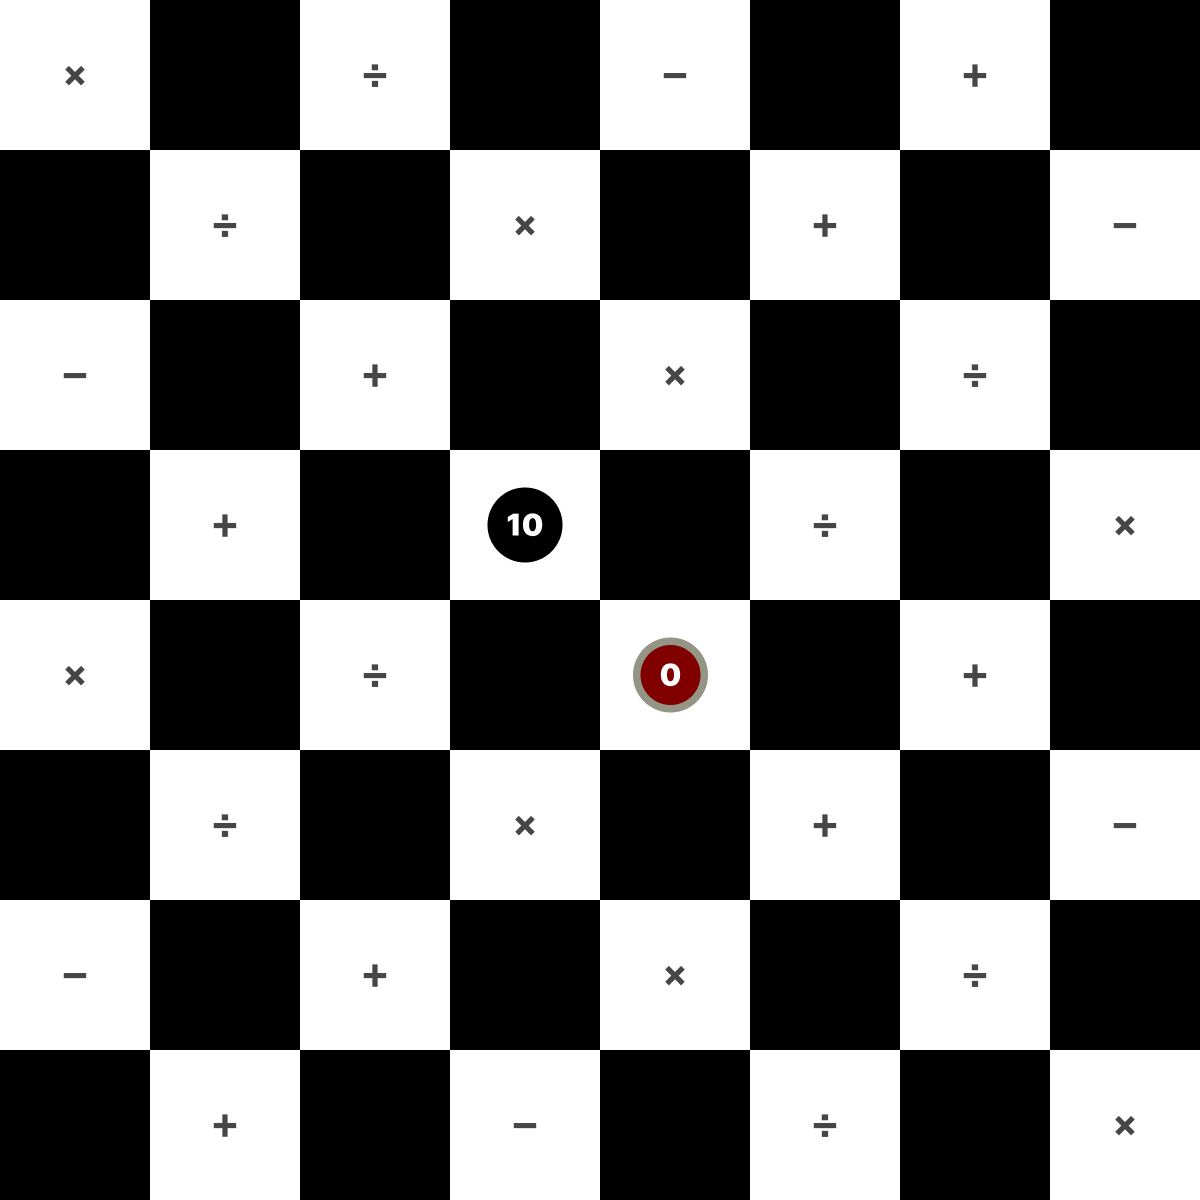
\includegraphics[width=0.4\linewidth]{images/example_state.png}\end{gathered}\right) = \resizebox{0.4\textwidth}{!}{$\begin{bmatrix}
            \rz & \gz & \gz & \gz & \gz & \gz & \gz & \gz & \gz & \gz & \gz & \gz & \gz & \gz & \gz & \gs & \gz & \go & \gz & \gz & \gz & \gz \\
            \rz & \gz & \gz & \gz & \gz & \gz & \gz & \gz & \gz & \gz & \gz & \gz & \gz & \gz & \gz & \gs & \gz & \gz & \go & \gz & \gz & \gz \\
            \rz & \gz & \gz & \gz & \gz & \gz & \gz & \gz & \gz & \gz & \gz & \gz & \gz & \gz & \gz & \gs & \gz & \gz & \gz & \gz & \go & \gz \\
            \rz & \gz & \gz & \gz & \gz & \gz & \gz & \gz & \gz & \gz & \gz & \gz & \gz & \gz & \gz & \gs & \gz & \gz & \gz & \go & \gz & \gz \\
            \rz & \gz & \gz & \gz & \gz & \gz & \gz & \gz & \gz & \gz & \gz & \gz & \gz & \gz & \gz & \gs & \gz & \gz & \go & \gz & \gz & \gz \\
            \rz & \gz & \gz & \gz & \gz & \gz & \gz & \gz & \gz & \gz & \gz & \gz & \gz & \gz & \gz & \gs & \gz & \go & \gz & \gz & \gz & \gz \\
            \rz & \gz & \gz & \gz & \gz & \gz & \gz & \gz & \gz & \gz & \gz & \gz & \gz & \gz & \gz & \gs & \gz & \gz & \gz & \go & \gz & \gz \\
            \rz & \gz & \gz & \gz & \gz & \gz & \gz & \gz & \gz & \gz & \gz & \gz & \gz & \gz & \gz & \gs & \gz & \gz & \gz & \gz & \go & \gz \\
            \rz & \gz & \gz & \gz & \gz & \gz & \gz & \gz & \gz & \gz & \gz & \gz & \gz & \gz & \gz & \gs & \gz & \gz & \gz & \gz & \go & \gz \\
            \rz & \gz & \gz & \gz & \gz & \gz & \gz & \gz & \gz & \gz & \gz & \gz & \gz & \gz & \gz & \gs & \gz & \gz & \gz & \go & \gz & \gz \\
            \rz & \gz & \gz & \gz & \gz & \gz & \gz & \gz & \gz & \gz & \gz & \gz & \gz & \gz & \gz & \gs & \gz & \go & \gz & \gz & \gz & \gz \\
            \rz & \gz & \gz & \gz & \gz & \gz & \gz & \gz & \gz & \gz & \gz & \gz & \gz & \gz & \gz & \gs & \gz & \gz & \go & \gz & \gz & \gz \\
            \rz & \gz & \gz & \gz & \gz & \gz & \gz & \gz & \gz & \gz & \gz & \gz & \gz & \gz & \gz & \gs & \gz & \gz & \gz & \go & \gz & \gz \\
            \rz & \gz & \gz & \gz & \gz & \gz & \gz & \gz & \gz & \gz & \gz & \gz & \gz & \gz & \gz & \gs & \gz & \gz & \gz & \gz & \go & \gz \\
            \rz & \go & \gz & \gz & \gz & \gz & \gz & \gz & \gz & \gz & \gz & \gz & \gz & \go & \go & \gs & \gz & \gz & \go & \gz & \gz & \go \\
            \rz & \gz & \gz & \gz & \gz & \gz & \gz & \gz & \gz & \gz & \gz & \gz & \gz & \gz & \gz & \gs & \gz & \go & \gz & \gz & \gz & \gz \\
            \rz & \gz & \gz & \gz & \gz & \gz & \gz & \gz & \gz & \gz & \gz & \gz & \gz & \gz & \gz & \gs & \gz & \go & \gz & \gz & \gz & \gz \\
            \rz & \gz & \gz & \gz & \gz & \gz & \gz & \gz & \gz & \gz & \gz & \go & \gz & \gz & \gz & \gs & \gz & \gz & \go & \gz & \gz & \gz \\
            \rz & \gz & \gz & \gz & \gz & \gz & \gz & \gz & \gz & \gz & \gz & \gz & \gz & \gz & \gz & \gs & \gz & \gz & \gz & \gz & \go & \gz \\
            \rz & \gz & \gz & \gz & \gz & \gz & \gz & \gz & \gz & \gz & \gz & \gz & \gz & \gz & \gz & \gs & \gz & \gz & \gz & \go & \gz & \gz \\
            \rz & \gz & \gz & \gz & \gz & \gz & \gz & \gz & \gz & \gz & \gz & \gz & \gz & \gz & \gz & \gs & \gz & \gz & \go & \gz & \gz & \gz \\
            \rz & \gz & \gz & \gz & \gz & \gz & \gz & \gz & \gz & \gz & \gz & \gz & \gz & \gz & \gz & \gs & \gz & \go & \gz & \gz & \gz & \gz \\
            \rz & \gz & \gz & \gz & \gz & \gz & \gz & \gz & \gz & \gz & \gz & \gz & \gz & \gz & \gz & \gs & \gz & \gz & \gz & \go & \gz & \gz \\
            \rz & \gz & \gz & \gz & \gz & \gz & \gz & \gz & \gz & \gz & \gz & \gz & \gz & \gz & \gz & \gs & \gz & \gz & \gz & \gz & \go & \gz \\
            \rz & \gz & \gz & \gz & \gz & \gz & \gz & \gz & \gz & \gz & \gz & \gz & \gz & \gz & \gz & \gs & \gz & \gz & \gz & \gz & \go & \gz \\
            \rz & \gz & \gz & \gz & \gz & \gz & \gz & \gz & \gz & \gz & \gz & \gz & \gz & \gz & \gz & \gs & \gz & \gz & \gz & \go & \gz & \gz \\
            \rz & \gz & \gz & \gz & \gz & \gz & \gz & \gz & \gz & \gz & \gz & \gz & \gz & \gz & \gz & \gs & \gz & \go & \gz & \gz & \gz & \gz \\
            \rz & \gz & \gz & \gz & \gz & \gz & \gz & \gz & \gz & \gz & \gz & \gz & \gz & \gz & \gz & \gs & \gz & \gz & \go & \gz & \gz & \gz \\
            \rz & \gz & \gz & \gz & \gz & \gz & \gz & \gz & \gz & \gz & \gz & \gz & \gz & \gz & \gz & \gs & \gz & \gz & \gz & \go & \gz & \gz \\
            \rz & \gz & \gz & \gz & \gz & \gz & \gz & \gz & \gz & \gz & \gz & \gz & \gz & \gz & \gz & \gs & \gz & \gz & \gz & \gz & \go & \gz \\
            \rz & \gz & \gz & \gz & \gz & \gz & \gz & \gz & \gz & \gz & \gz & \gz & \gz & \gz & \gz & \gs & \gz & \gz & \go & \gz & \gz & \gz \\
            \rz & \gz & \gz & \gz & \gz & \gz & \gz & \gz & \gz & \gz & \gz & \gz & \gz & \gz & \gz & \gs & \gz & \go & \gz & \gz & \gz & \gz
        \end{bmatrix}$}
    \end{equation*}
    \caption{Example State Representation with the Current Player Highlighted}
    \label{fig:example-state-representation-first}
\end{figure}

The second to fourteenth column represents the one-hot encoding of the value of the current piece in the cell as shown as red cells in the example shown in Figure \ref{fig:example-state-representation-second-fourteenth}. The values of these columns are all zero if there is currently no piece in the cell. Twelve dimensions are used to represent one of the twelve different values a piece may have. The values of all of these dimensions are zero except for a single dimension that has a value of one if it corresponds to the value of the current piece on the cell.

\begin{figure}[H]
    \begin{equation*} 
        \verb|Encode|\left(\begin{gathered}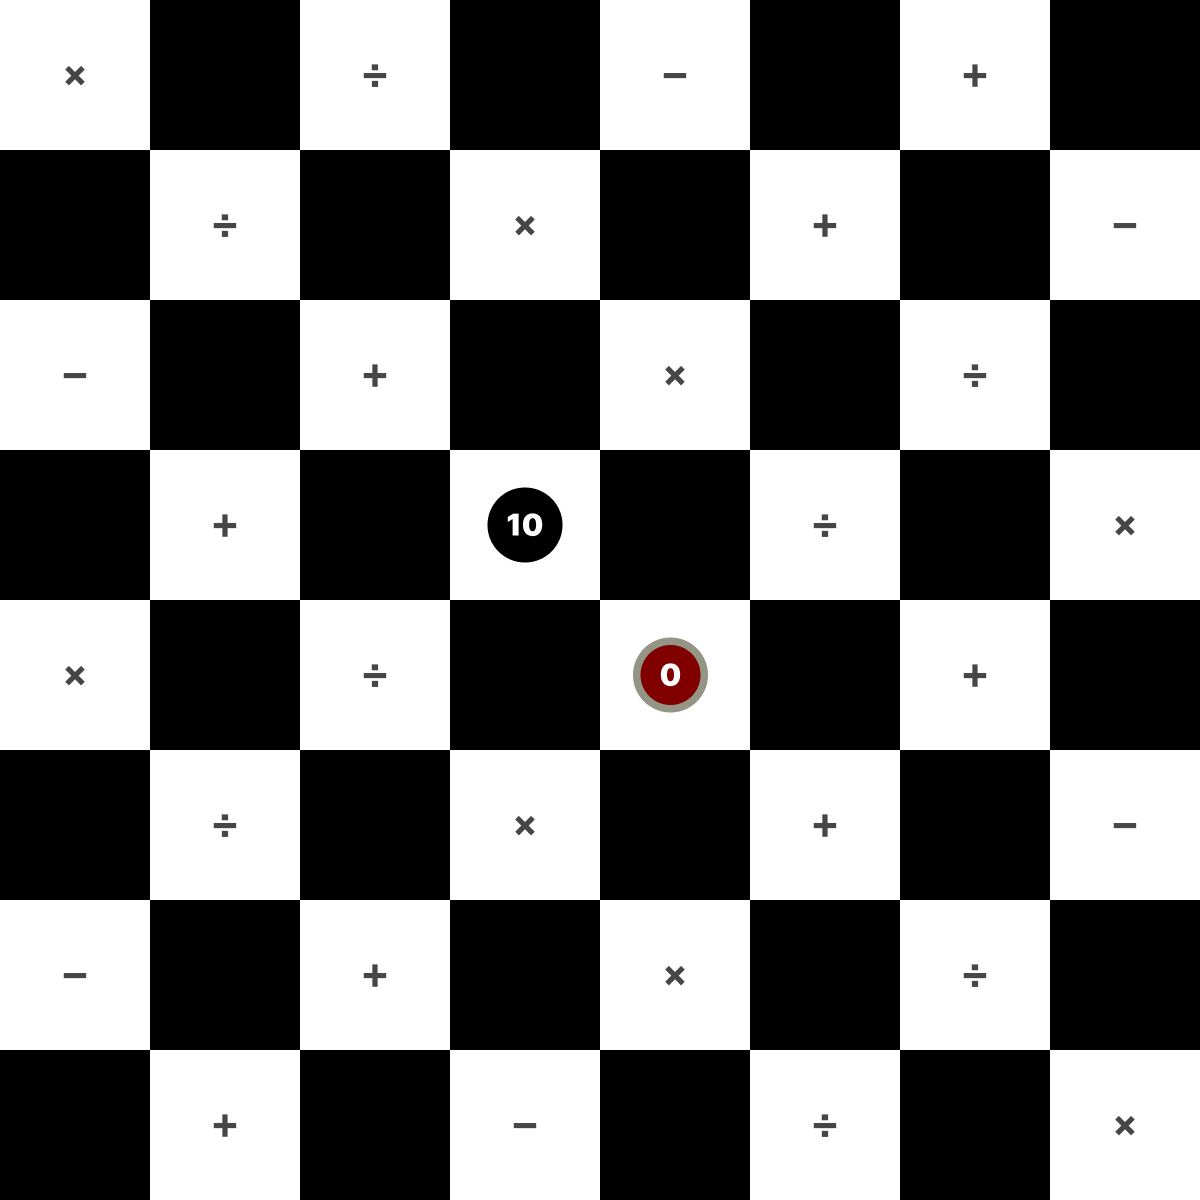
\includegraphics[width=0.4\linewidth]{images/example_state.png}\end{gathered}\right) = \resizebox{0.4\textwidth}{!}{$\begin{bmatrix}
            \gz & \rz & \rz & \rz & \rz & \rz & \rz & \rz & \rz & \rz & \rz & \rz & \rz & \gz & \gz & \gs & \gz & \go & \gz & \gz & \gz & \gz \\
            \gz & \rz & \rz & \rz & \rz & \rz & \rz & \rz & \rz & \rz & \rz & \rz & \rz & \gz & \gz & \gs & \gz & \gz & \go & \gz & \gz & \gz \\
            \gz & \rz & \rz & \rz & \rz & \rz & \rz & \rz & \rz & \rz & \rz & \rz & \rz & \gz & \gz & \gs & \gz & \gz & \gz & \gz & \go & \gz \\
            \gz & \rz & \rz & \rz & \rz & \rz & \rz & \rz & \rz & \rz & \rz & \rz & \rz & \gz & \gz & \gs & \gz & \gz & \gz & \go & \gz & \gz \\
            \gz & \rz & \rz & \rz & \rz & \rz & \rz & \rz & \rz & \rz & \rz & \rz & \rz & \gz & \gz & \gs & \gz & \gz & \go & \gz & \gz & \gz \\
            \gz & \rz & \rz & \rz & \rz & \rz & \rz & \rz & \rz & \rz & \rz & \rz & \rz & \gz & \gz & \gs & \gz & \go & \gz & \gz & \gz & \gz \\
            \gz & \rz & \rz & \rz & \rz & \rz & \rz & \rz & \rz & \rz & \rz & \rz & \rz & \gz & \gz & \gs & \gz & \gz & \gz & \go & \gz & \gz \\
            \gz & \rz & \rz & \rz & \rz & \rz & \rz & \rz & \rz & \rz & \rz & \rz & \rz & \gz & \gz & \gs & \gz & \gz & \gz & \gz & \go & \gz \\
            \gz & \rz & \rz & \rz & \rz & \rz & \rz & \rz & \rz & \rz & \rz & \rz & \rz & \gz & \gz & \gs & \gz & \gz & \gz & \gz & \go & \gz \\
            \gz & \rz & \rz & \rz & \rz & \rz & \rz & \rz & \rz & \rz & \rz & \rz & \rz & \gz & \gz & \gs & \gz & \gz & \gz & \go & \gz & \gz \\
            \gz & \rz & \rz & \rz & \rz & \rz & \rz & \rz & \rz & \rz & \rz & \rz & \rz & \gz & \gz & \gs & \gz & \go & \gz & \gz & \gz & \gz \\
            \gz & \rz & \rz & \rz & \rz & \rz & \rz & \rz & \rz & \rz & \rz & \rz & \rz & \gz & \gz & \gs & \gz & \gz & \go & \gz & \gz & \gz \\
            \gz & \rz & \rz & \rz & \rz & \rz & \rz & \rz & \rz & \rz & \rz & \rz & \rz & \gz & \gz & \gs & \gz & \gz & \gz & \go & \gz & \gz \\
            \gz & \rz & \rz & \rz & \rz & \rz & \rz & \rz & \rz & \rz & \rz & \rz & \rz & \gz & \gz & \gs & \gz & \gz & \gz & \gz & \go & \gz \\
            \gz & \ro & \rz & \rz & \rz & \rz & \rz & \rz & \rz & \rz & \rz & \rz & \rz & \go & \go & \gs & \gz & \gz & \go & \gz & \gz & \go \\
            \gz & \rz & \rz & \rz & \rz & \rz & \rz & \rz & \rz & \rz & \rz & \rz & \rz & \gz & \gz & \gs & \gz & \go & \gz & \gz & \gz & \gz \\
            \gz & \rz & \rz & \rz & \rz & \rz & \rz & \rz & \rz & \rz & \rz & \rz & \rz & \gz & \gz & \gs & \gz & \go & \gz & \gz & \gz & \gz \\
            \gz & \rz & \rz & \rz & \rz & \rz & \rz & \rz & \rz & \rz & \rz & \ro & \rz & \gz & \gz & \gs & \gz & \gz & \go & \gz & \gz & \gz \\
            \gz & \rz & \rz & \rz & \rz & \rz & \rz & \rz & \rz & \rz & \rz & \rz & \rz & \gz & \gz & \gs & \gz & \gz & \gz & \gz & \go & \gz \\
            \gz & \rz & \rz & \rz & \rz & \rz & \rz & \rz & \rz & \rz & \rz & \rz & \rz & \gz & \gz & \gs & \gz & \gz & \gz & \go & \gz & \gz \\
            \gz & \rz & \rz & \rz & \rz & \rz & \rz & \rz & \rz & \rz & \rz & \rz & \rz & \gz & \gz & \gs & \gz & \gz & \go & \gz & \gz & \gz \\
            \gz & \rz & \rz & \rz & \rz & \rz & \rz & \rz & \rz & \rz & \rz & \rz & \rz & \gz & \gz & \gs & \gz & \go & \gz & \gz & \gz & \gz \\
            \gz & \rz & \rz & \rz & \rz & \rz & \rz & \rz & \rz & \rz & \rz & \rz & \rz & \gz & \gz & \gs & \gz & \gz & \gz & \go & \gz & \gz \\
            \gz & \rz & \rz & \rz & \rz & \rz & \rz & \rz & \rz & \rz & \rz & \rz & \rz & \gz & \gz & \gs & \gz & \gz & \gz & \gz & \go & \gz \\
            \gz & \rz & \rz & \rz & \rz & \rz & \rz & \rz & \rz & \rz & \rz & \rz & \rz & \gz & \gz & \gs & \gz & \gz & \gz & \gz & \go & \gz \\
            \gz & \rz & \rz & \rz & \rz & \rz & \rz & \rz & \rz & \rz & \rz & \rz & \rz & \gz & \gz & \gs & \gz & \gz & \gz & \go & \gz & \gz \\
            \gz & \rz & \rz & \rz & \rz & \rz & \rz & \rz & \rz & \rz & \rz & \rz & \rz & \gz & \gz & \gs & \gz & \go & \gz & \gz & \gz & \gz \\
            \gz & \rz & \rz & \rz & \rz & \rz & \rz & \rz & \rz & \rz & \rz & \rz & \rz & \gz & \gz & \gs & \gz & \gz & \go & \gz & \gz & \gz \\
            \gz & \rz & \rz & \rz & \rz & \rz & \rz & \rz & \rz & \rz & \rz & \rz & \rz & \gz & \gz & \gs & \gz & \gz & \gz & \go & \gz & \gz \\
            \gz & \rz & \rz & \rz & \rz & \rz & \rz & \rz & \rz & \rz & \rz & \rz & \rz & \gz & \gz & \gs & \gz & \gz & \gz & \gz & \go & \gz \\
            \gz & \rz & \rz & \rz & \rz & \rz & \rz & \rz & \rz & \rz & \rz & \rz & \rz & \gz & \gz & \gs & \gz & \gz & \go & \gz & \gz & \gz \\
            \gz & \rz & \rz & \rz & \rz & \rz & \rz & \rz & \rz & \rz & \rz & \rz & \rz & \gz & \gz & \gs & \gz & \go & \gz & \gz & \gz & \gz
        \end{bmatrix}$}
    \end{equation*}
    \caption{Example State Representation with the Current Piece Type Highlighted}
    \label{fig:example-state-representation-second-fourteenth}
\end{figure}

The fifteenth column represents the dama status of the current piece in the cell as shown as red cells in the example shown in Figure \ref{fig:example-state-representation-fifteenth}. The value of this column is zero if the current piece on the cell is a normal piece and one if the current piece on the cell is a dama piece. This column tells whether the current piece on the cell is a dama piece that can move in all four directions and move more than one distance at a time or not.

\begin{figure}[H]
    \begin{equation*} 
        \verb|Encode|\left(\begin{gathered}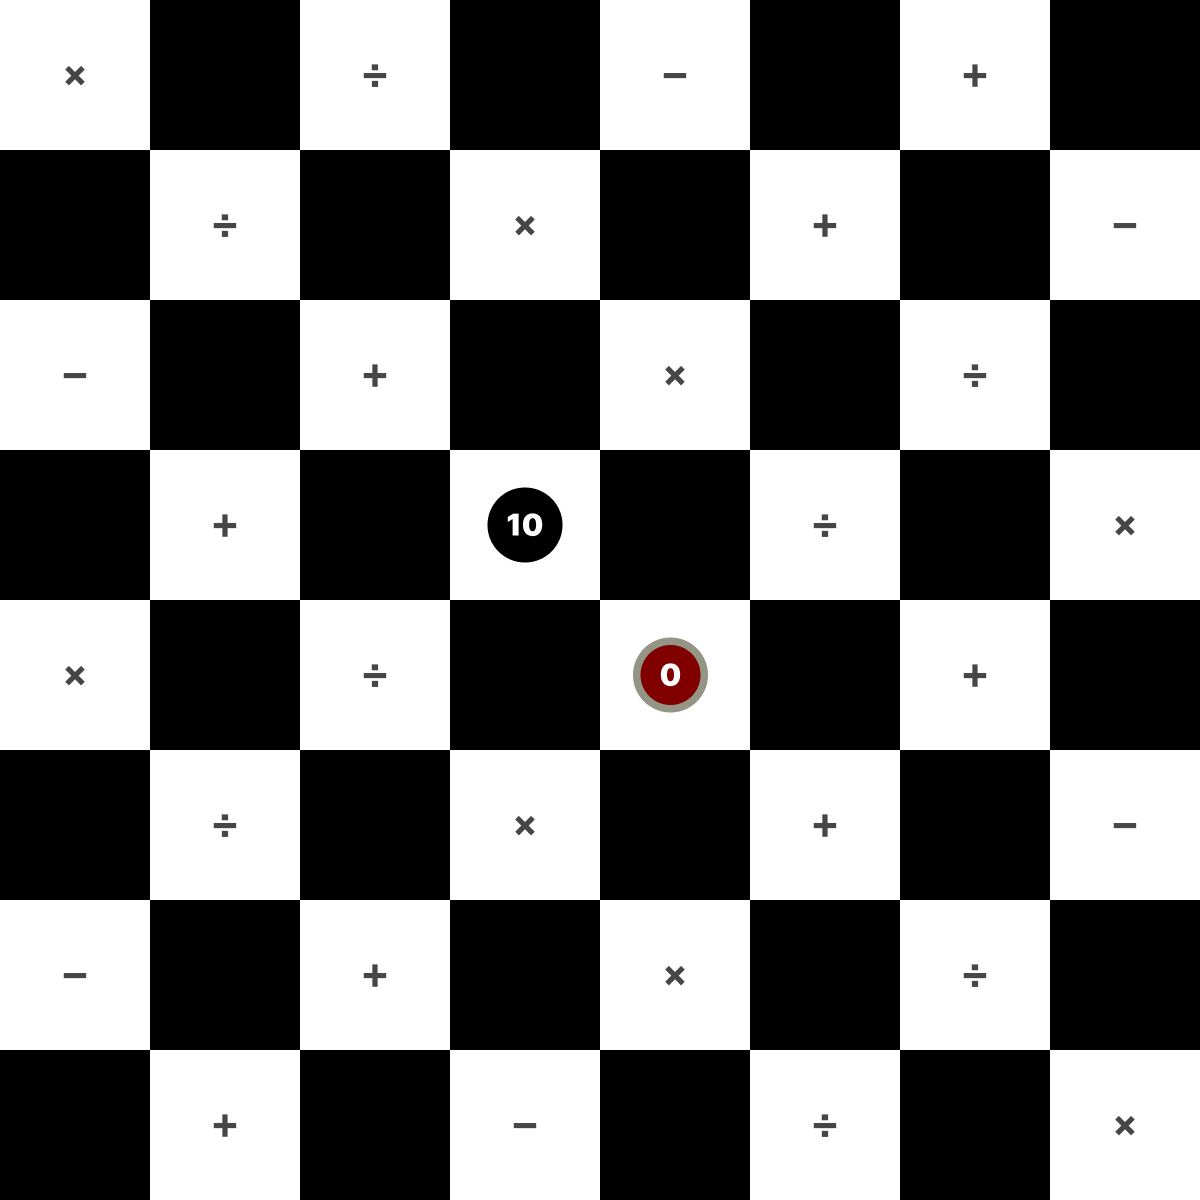
\includegraphics[width=0.4\linewidth]{images/example_state.png}\end{gathered}\right) = \resizebox{0.4\textwidth}{!}{$\begin{bmatrix}
            \gz & \gz & \gz & \gz & \gz & \gz & \gz & \gz & \gz & \gz & \gz & \gz & \gz & \rz & \gz & \gs & \gz & \go & \gz & \gz & \gz & \gz \\
            \gz & \gz & \gz & \gz & \gz & \gz & \gz & \gz & \gz & \gz & \gz & \gz & \gz & \rz & \gz & \gs & \gz & \gz & \go & \gz & \gz & \gz \\
            \gz & \gz & \gz & \gz & \gz & \gz & \gz & \gz & \gz & \gz & \gz & \gz & \gz & \rz & \gz & \gs & \gz & \gz & \gz & \gz & \go & \gz \\
            \gz & \gz & \gz & \gz & \gz & \gz & \gz & \gz & \gz & \gz & \gz & \gz & \gz & \rz & \gz & \gs & \gz & \gz & \gz & \go & \gz & \gz \\
            \gz & \gz & \gz & \gz & \gz & \gz & \gz & \gz & \gz & \gz & \gz & \gz & \gz & \rz & \gz & \gs & \gz & \gz & \go & \gz & \gz & \gz \\
            \gz & \gz & \gz & \gz & \gz & \gz & \gz & \gz & \gz & \gz & \gz & \gz & \gz & \rz & \gz & \gs & \gz & \go & \gz & \gz & \gz & \gz \\
            \gz & \gz & \gz & \gz & \gz & \gz & \gz & \gz & \gz & \gz & \gz & \gz & \gz & \rz & \gz & \gs & \gz & \gz & \gz & \go & \gz & \gz \\
            \gz & \gz & \gz & \gz & \gz & \gz & \gz & \gz & \gz & \gz & \gz & \gz & \gz & \rz & \gz & \gs & \gz & \gz & \gz & \gz & \go & \gz \\
            \gz & \gz & \gz & \gz & \gz & \gz & \gz & \gz & \gz & \gz & \gz & \gz & \gz & \rz & \gz & \gs & \gz & \gz & \gz & \gz & \go & \gz \\
            \gz & \gz & \gz & \gz & \gz & \gz & \gz & \gz & \gz & \gz & \gz & \gz & \gz & \rz & \gz & \gs & \gz & \gz & \gz & \go & \gz & \gz \\
            \gz & \gz & \gz & \gz & \gz & \gz & \gz & \gz & \gz & \gz & \gz & \gz & \gz & \rz & \gz & \gs & \gz & \go & \gz & \gz & \gz & \gz \\
            \gz & \gz & \gz & \gz & \gz & \gz & \gz & \gz & \gz & \gz & \gz & \gz & \gz & \rz & \gz & \gs & \gz & \gz & \go & \gz & \gz & \gz \\
            \gz & \gz & \gz & \gz & \gz & \gz & \gz & \gz & \gz & \gz & \gz & \gz & \gz & \rz & \gz & \gs & \gz & \gz & \gz & \go & \gz & \gz \\
            \gz & \gz & \gz & \gz & \gz & \gz & \gz & \gz & \gz & \gz & \gz & \gz & \gz & \rz & \gz & \gs & \gz & \gz & \gz & \gz & \go & \gz \\
            \gz & \go & \gz & \gz & \gz & \gz & \gz & \gz & \gz & \gz & \gz & \gz & \gz & \ro & \go & \gs & \gz & \gz & \go & \gz & \gz & \go \\
            \gz & \gz & \gz & \gz & \gz & \gz & \gz & \gz & \gz & \gz & \gz & \gz & \gz & \rz & \gz & \gs & \gz & \go & \gz & \gz & \gz & \gz \\
            \gz & \gz & \gz & \gz & \gz & \gz & \gz & \gz & \gz & \gz & \gz & \gz & \gz & \rz & \gz & \gs & \gz & \go & \gz & \gz & \gz & \gz \\
            \gz & \gz & \gz & \gz & \gz & \gz & \gz & \gz & \gz & \gz & \gz & \go & \gz & \rz & \gz & \gs & \gz & \gz & \go & \gz & \gz & \gz \\
            \gz & \gz & \gz & \gz & \gz & \gz & \gz & \gz & \gz & \gz & \gz & \gz & \gz & \rz & \gz & \gs & \gz & \gz & \gz & \gz & \go & \gz \\
            \gz & \gz & \gz & \gz & \gz & \gz & \gz & \gz & \gz & \gz & \gz & \gz & \gz & \rz & \gz & \gs & \gz & \gz & \gz & \go & \gz & \gz \\
            \gz & \gz & \gz & \gz & \gz & \gz & \gz & \gz & \gz & \gz & \gz & \gz & \gz & \rz & \gz & \gs & \gz & \gz & \go & \gz & \gz & \gz \\
            \gz & \gz & \gz & \gz & \gz & \gz & \gz & \gz & \gz & \gz & \gz & \gz & \gz & \rz & \gz & \gs & \gz & \go & \gz & \gz & \gz & \gz \\
            \gz & \gz & \gz & \gz & \gz & \gz & \gz & \gz & \gz & \gz & \gz & \gz & \gz & \rz & \gz & \gs & \gz & \gz & \gz & \go & \gz & \gz \\
            \gz & \gz & \gz & \gz & \gz & \gz & \gz & \gz & \gz & \gz & \gz & \gz & \gz & \rz & \gz & \gs & \gz & \gz & \gz & \gz & \go & \gz \\
            \gz & \gz & \gz & \gz & \gz & \gz & \gz & \gz & \gz & \gz & \gz & \gz & \gz & \rz & \gz & \gs & \gz & \gz & \gz & \gz & \go & \gz \\
            \gz & \gz & \gz & \gz & \gz & \gz & \gz & \gz & \gz & \gz & \gz & \gz & \gz & \rz & \gz & \gs & \gz & \gz & \gz & \go & \gz & \gz \\
            \gz & \gz & \gz & \gz & \gz & \gz & \gz & \gz & \gz & \gz & \gz & \gz & \gz & \rz & \gz & \gs & \gz & \go & \gz & \gz & \gz & \gz \\
            \gz & \gz & \gz & \gz & \gz & \gz & \gz & \gz & \gz & \gz & \gz & \gz & \gz & \rz & \gz & \gs & \gz & \gz & \go & \gz & \gz & \gz \\
            \gz & \gz & \gz & \gz & \gz & \gz & \gz & \gz & \gz & \gz & \gz & \gz & \gz & \rz & \gz & \gs & \gz & \gz & \gz & \go & \gz & \gz \\
            \gz & \gz & \gz & \gz & \gz & \gz & \gz & \gz & \gz & \gz & \gz & \gz & \gz & \rz & \gz & \gs & \gz & \gz & \gz & \gz & \go & \gz \\
            \gz & \gz & \gz & \gz & \gz & \gz & \gz & \gz & \gz & \gz & \gz & \gz & \gz & \rz & \gz & \gs & \gz & \gz & \go & \gz & \gz & \gz \\
            \gz & \gz & \gz & \gz & \gz & \gz & \gz & \gz & \gz & \gz & \gz & \gz & \gz & \rz & \gz & \gs & \gz & \go & \gz & \gz & \gz & \gz
        \end{bmatrix}$}
    \end{equation*}
    \caption{Example State Representation with the Dama Status Highlighted}
    \label{fig:example-state-representation-fifteenth}
\end{figure}

The sixteenth column represents the owner of the piece in the current cell as shown as red cells in the example shown in Figure \ref{fig:example-state-representation-sixteenth}. The value of this column is one if the current player owns the piece in the current cell and zero if not. This column tells whether the current player owns the piece in the current cell and can make a valid move with it.

\begin{figure}[H]
    \begin{equation*} 
        \verb|Encode|\left(\begin{gathered}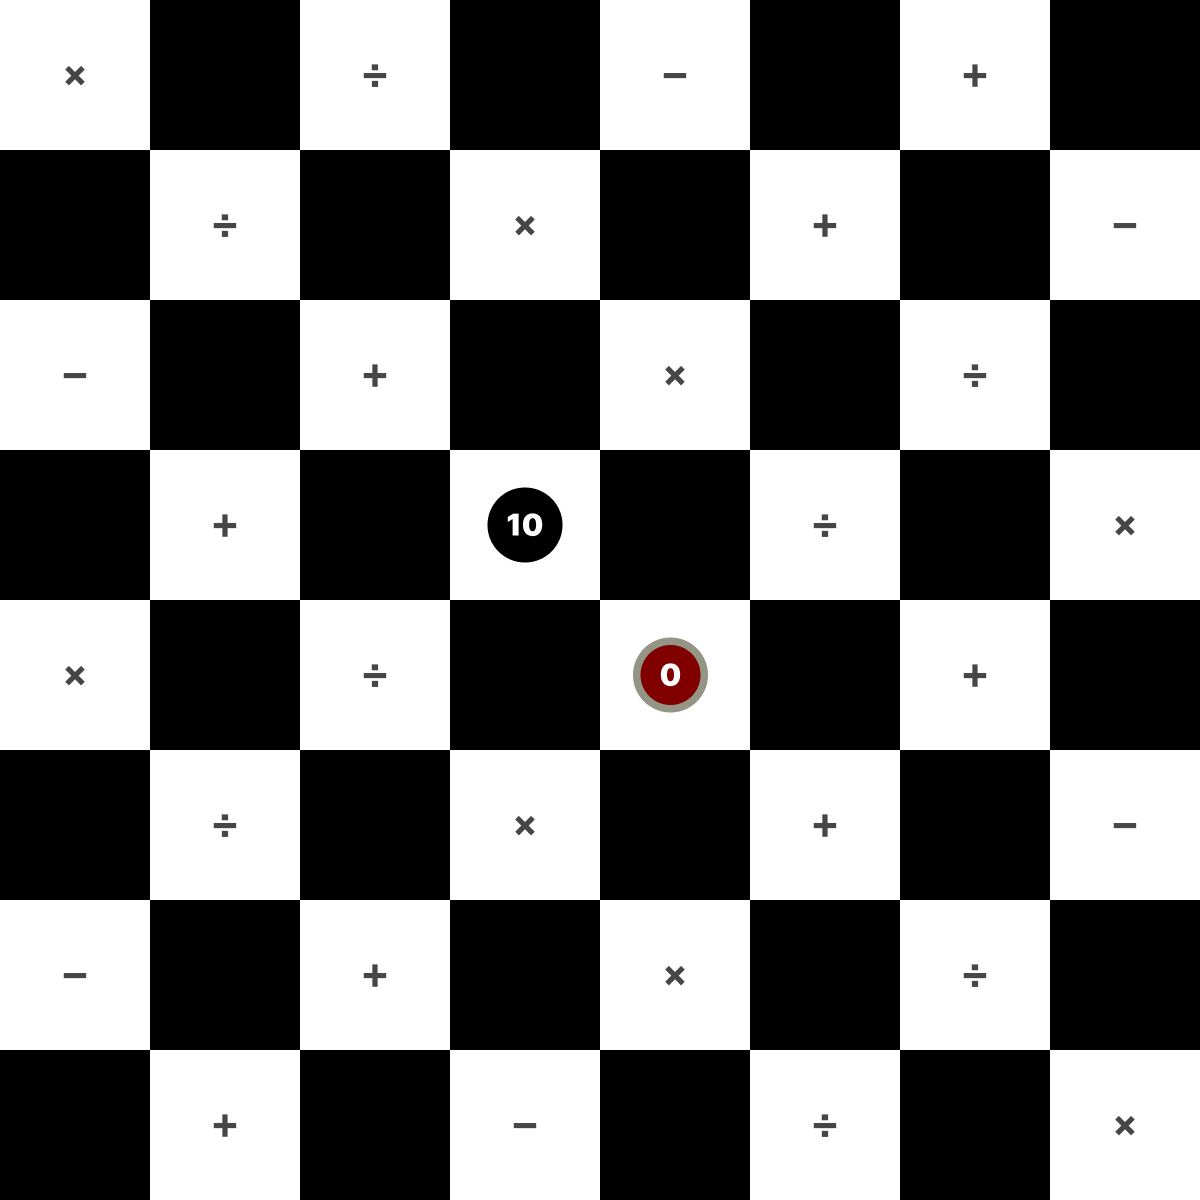
\includegraphics[width=0.4\linewidth]{images/example_state.png}\end{gathered}\right) = \resizebox{0.4\textwidth}{!}{$\begin{bmatrix}
            \gz & \gz & \gz & \gz & \gz & \gz & \gz & \gz & \gz & \gz & \gz & \gz & \gz & \gz & \rz & \gs & \gz & \go & \gz & \gz & \gz & \gz \\
            \gz & \gz & \gz & \gz & \gz & \gz & \gz & \gz & \gz & \gz & \gz & \gz & \gz & \gz & \rz & \gs & \gz & \gz & \go & \gz & \gz & \gz \\
            \gz & \gz & \gz & \gz & \gz & \gz & \gz & \gz & \gz & \gz & \gz & \gz & \gz & \gz & \rz & \gs & \gz & \gz & \gz & \gz & \go & \gz \\
            \gz & \gz & \gz & \gz & \gz & \gz & \gz & \gz & \gz & \gz & \gz & \gz & \gz & \gz & \rz & \gs & \gz & \gz & \gz & \go & \gz & \gz \\
            \gz & \gz & \gz & \gz & \gz & \gz & \gz & \gz & \gz & \gz & \gz & \gz & \gz & \gz & \rz & \gs & \gz & \gz & \go & \gz & \gz & \gz \\
            \gz & \gz & \gz & \gz & \gz & \gz & \gz & \gz & \gz & \gz & \gz & \gz & \gz & \gz & \rz & \gs & \gz & \go & \gz & \gz & \gz & \gz \\
            \gz & \gz & \gz & \gz & \gz & \gz & \gz & \gz & \gz & \gz & \gz & \gz & \gz & \gz & \rz & \gs & \gz & \gz & \gz & \go & \gz & \gz \\
            \gz & \gz & \gz & \gz & \gz & \gz & \gz & \gz & \gz & \gz & \gz & \gz & \gz & \gz & \rz & \gs & \gz & \gz & \gz & \gz & \go & \gz \\
            \gz & \gz & \gz & \gz & \gz & \gz & \gz & \gz & \gz & \gz & \gz & \gz & \gz & \gz & \rz & \gs & \gz & \gz & \gz & \gz & \go & \gz \\
            \gz & \gz & \gz & \gz & \gz & \gz & \gz & \gz & \gz & \gz & \gz & \gz & \gz & \gz & \rz & \gs & \gz & \gz & \gz & \go & \gz & \gz \\
            \gz & \gz & \gz & \gz & \gz & \gz & \gz & \gz & \gz & \gz & \gz & \gz & \gz & \gz & \rz & \gs & \gz & \go & \gz & \gz & \gz & \gz \\
            \gz & \gz & \gz & \gz & \gz & \gz & \gz & \gz & \gz & \gz & \gz & \gz & \gz & \gz & \rz & \gs & \gz & \gz & \go & \gz & \gz & \gz \\
            \gz & \gz & \gz & \gz & \gz & \gz & \gz & \gz & \gz & \gz & \gz & \gz & \gz & \gz & \rz & \gs & \gz & \gz & \gz & \go & \gz & \gz \\
            \gz & \gz & \gz & \gz & \gz & \gz & \gz & \gz & \gz & \gz & \gz & \gz & \gz & \gz & \rz & \gs & \gz & \gz & \gz & \gz & \go & \gz \\
            \gz & \go & \gz & \gz & \gz & \gz & \gz & \gz & \gz & \gz & \gz & \gz & \gz & \go & \ro & \gs & \gz & \gz & \go & \gz & \gz & \go \\
            \gz & \gz & \gz & \gz & \gz & \gz & \gz & \gz & \gz & \gz & \gz & \gz & \gz & \gz & \rz & \gs & \gz & \go & \gz & \gz & \gz & \gz \\
            \gz & \gz & \gz & \gz & \gz & \gz & \gz & \gz & \gz & \gz & \gz & \gz & \gz & \gz & \rz & \gs & \gz & \go & \gz & \gz & \gz & \gz \\
            \gz & \gz & \gz & \gz & \gz & \gz & \gz & \gz & \gz & \gz & \gz & \go & \gz & \gz & \rz & \gs & \gz & \gz & \go & \gz & \gz & \gz \\
            \gz & \gz & \gz & \gz & \gz & \gz & \gz & \gz & \gz & \gz & \gz & \gz & \gz & \gz & \rz & \gs & \gz & \gz & \gz & \gz & \go & \gz \\
            \gz & \gz & \gz & \gz & \gz & \gz & \gz & \gz & \gz & \gz & \gz & \gz & \gz & \gz & \rz & \gs & \gz & \gz & \gz & \go & \gz & \gz \\
            \gz & \gz & \gz & \gz & \gz & \gz & \gz & \gz & \gz & \gz & \gz & \gz & \gz & \gz & \rz & \gs & \gz & \gz & \go & \gz & \gz & \gz \\
            \gz & \gz & \gz & \gz & \gz & \gz & \gz & \gz & \gz & \gz & \gz & \gz & \gz & \gz & \rz & \gs & \gz & \go & \gz & \gz & \gz & \gz \\
            \gz & \gz & \gz & \gz & \gz & \gz & \gz & \gz & \gz & \gz & \gz & \gz & \gz & \gz & \rz & \gs & \gz & \gz & \gz & \go & \gz & \gz \\
            \gz & \gz & \gz & \gz & \gz & \gz & \gz & \gz & \gz & \gz & \gz & \gz & \gz & \gz & \rz & \gs & \gz & \gz & \gz & \gz & \go & \gz \\
            \gz & \gz & \gz & \gz & \gz & \gz & \gz & \gz & \gz & \gz & \gz & \gz & \gz & \gz & \rz & \gs & \gz & \gz & \gz & \gz & \go & \gz \\
            \gz & \gz & \gz & \gz & \gz & \gz & \gz & \gz & \gz & \gz & \gz & \gz & \gz & \gz & \rz & \gs & \gz & \gz & \gz & \go & \gz & \gz \\
            \gz & \gz & \gz & \gz & \gz & \gz & \gz & \gz & \gz & \gz & \gz & \gz & \gz & \gz & \rz & \gs & \gz & \go & \gz & \gz & \gz & \gz \\
            \gz & \gz & \gz & \gz & \gz & \gz & \gz & \gz & \gz & \gz & \gz & \gz & \gz & \gz & \rz & \gs & \gz & \gz & \go & \gz & \gz & \gz \\
            \gz & \gz & \gz & \gz & \gz & \gz & \gz & \gz & \gz & \gz & \gz & \gz & \gz & \gz & \rz & \gs & \gz & \gz & \gz & \go & \gz & \gz \\
            \gz & \gz & \gz & \gz & \gz & \gz & \gz & \gz & \gz & \gz & \gz & \gz & \gz & \gz & \rz & \gs & \gz & \gz & \gz & \gz & \go & \gz \\
            \gz & \gz & \gz & \gz & \gz & \gz & \gz & \gz & \gz & \gz & \gz & \gz & \gz & \gz & \rz & \gs & \gz & \gz & \go & \gz & \gz & \gz \\
            \gz & \gz & \gz & \gz & \gz & \gz & \gz & \gz & \gz & \gz & \gz & \gz & \gz & \gz & \rz & \gs & \gz & \go & \gz & \gz & \gz & \gz
        \end{bmatrix}$}
    \end{equation*}
    \caption{Example State Representation with the Piece Owner Highlighted}
    \label{fig:example-state-representation-sixteenth}
\end{figure}

The seventeenth column represents the relative score of the current player as shown as red cells in the example shown in Figure \ref{fig:example-state-representation-seventeenth}. This column is the same for all cells. A \verb|softmax| operation is applied first to the players' scores making them add up to one. The score of the current player after applying the \verb|softmax| operation is now relative to the sum of the player scores in the range of $0$ to $1$.

\begin{figure}[H]
    \begin{equation*} 
        \verb|Encode|\left(\begin{gathered}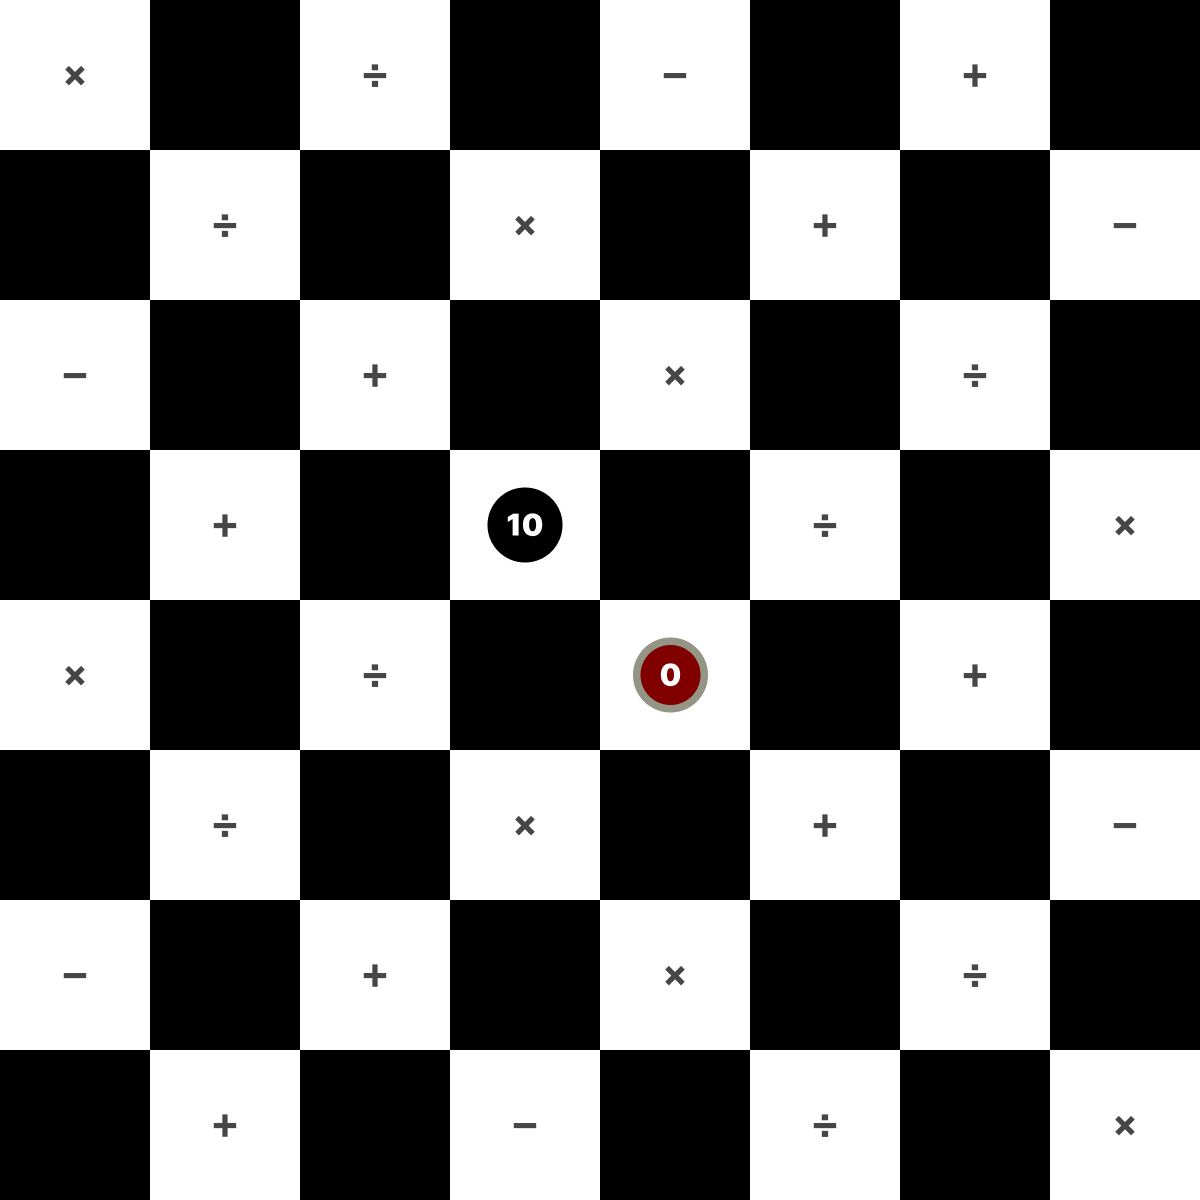
\includegraphics[width=0.4\linewidth]{images/example_state.png}\end{gathered}\right) = \resizebox{0.4\textwidth}{!}{$\begin{bmatrix}
            \gz & \gz & \gz & \gz & \gz & \gz & \gz & \gz & \gz & \gz & \gz & \gz & \gz & \gz & \gz & \rs & \gz & \go & \gz & \gz & \gz & \gz \\
            \gz & \gz & \gz & \gz & \gz & \gz & \gz & \gz & \gz & \gz & \gz & \gz & \gz & \gz & \gz & \rs & \gz & \gz & \go & \gz & \gz & \gz \\
            \gz & \gz & \gz & \gz & \gz & \gz & \gz & \gz & \gz & \gz & \gz & \gz & \gz & \gz & \gz & \rs & \gz & \gz & \gz & \gz & \go & \gz \\
            \gz & \gz & \gz & \gz & \gz & \gz & \gz & \gz & \gz & \gz & \gz & \gz & \gz & \gz & \gz & \rs & \gz & \gz & \gz & \go & \gz & \gz \\
            \gz & \gz & \gz & \gz & \gz & \gz & \gz & \gz & \gz & \gz & \gz & \gz & \gz & \gz & \gz & \rs & \gz & \gz & \go & \gz & \gz & \gz \\
            \gz & \gz & \gz & \gz & \gz & \gz & \gz & \gz & \gz & \gz & \gz & \gz & \gz & \gz & \gz & \rs & \gz & \go & \gz & \gz & \gz & \gz \\
            \gz & \gz & \gz & \gz & \gz & \gz & \gz & \gz & \gz & \gz & \gz & \gz & \gz & \gz & \gz & \rs & \gz & \gz & \gz & \go & \gz & \gz \\
            \gz & \gz & \gz & \gz & \gz & \gz & \gz & \gz & \gz & \gz & \gz & \gz & \gz & \gz & \gz & \rs & \gz & \gz & \gz & \gz & \go & \gz \\
            \gz & \gz & \gz & \gz & \gz & \gz & \gz & \gz & \gz & \gz & \gz & \gz & \gz & \gz & \gz & \rs & \gz & \gz & \gz & \gz & \go & \gz \\
            \gz & \gz & \gz & \gz & \gz & \gz & \gz & \gz & \gz & \gz & \gz & \gz & \gz & \gz & \gz & \rs & \gz & \gz & \gz & \go & \gz & \gz \\
            \gz & \gz & \gz & \gz & \gz & \gz & \gz & \gz & \gz & \gz & \gz & \gz & \gz & \gz & \gz & \rs & \gz & \go & \gz & \gz & \gz & \gz \\
            \gz & \gz & \gz & \gz & \gz & \gz & \gz & \gz & \gz & \gz & \gz & \gz & \gz & \gz & \gz & \rs & \gz & \gz & \go & \gz & \gz & \gz \\
            \gz & \gz & \gz & \gz & \gz & \gz & \gz & \gz & \gz & \gz & \gz & \gz & \gz & \gz & \gz & \rs & \gz & \gz & \gz & \go & \gz & \gz \\
            \gz & \gz & \gz & \gz & \gz & \gz & \gz & \gz & \gz & \gz & \gz & \gz & \gz & \gz & \gz & \rs & \gz & \gz & \gz & \gz & \go & \gz \\
            \gz & \go & \gz & \gz & \gz & \gz & \gz & \gz & \gz & \gz & \gz & \gz & \gz & \go & \go & \rs & \gz & \gz & \go & \gz & \gz & \go \\
            \gz & \gz & \gz & \gz & \gz & \gz & \gz & \gz & \gz & \gz & \gz & \gz & \gz & \gz & \gz & \rs & \gz & \go & \gz & \gz & \gz & \gz \\
            \gz & \gz & \gz & \gz & \gz & \gz & \gz & \gz & \gz & \gz & \gz & \gz & \gz & \gz & \gz & \rs & \gz & \go & \gz & \gz & \gz & \gz \\
            \gz & \gz & \gz & \gz & \gz & \gz & \gz & \gz & \gz & \gz & \gz & \go & \gz & \gz & \gz & \rs & \gz & \gz & \go & \gz & \gz & \gz \\
            \gz & \gz & \gz & \gz & \gz & \gz & \gz & \gz & \gz & \gz & \gz & \gz & \gz & \gz & \gz & \rs & \gz & \gz & \gz & \gz & \go & \gz \\
            \gz & \gz & \gz & \gz & \gz & \gz & \gz & \gz & \gz & \gz & \gz & \gz & \gz & \gz & \gz & \rs & \gz & \gz & \gz & \go & \gz & \gz \\
            \gz & \gz & \gz & \gz & \gz & \gz & \gz & \gz & \gz & \gz & \gz & \gz & \gz & \gz & \gz & \rs & \gz & \gz & \go & \gz & \gz & \gz \\
            \gz & \gz & \gz & \gz & \gz & \gz & \gz & \gz & \gz & \gz & \gz & \gz & \gz & \gz & \gz & \rs & \gz & \go & \gz & \gz & \gz & \gz \\
            \gz & \gz & \gz & \gz & \gz & \gz & \gz & \gz & \gz & \gz & \gz & \gz & \gz & \gz & \gz & \rs & \gz & \gz & \gz & \go & \gz & \gz \\
            \gz & \gz & \gz & \gz & \gz & \gz & \gz & \gz & \gz & \gz & \gz & \gz & \gz & \gz & \gz & \rs & \gz & \gz & \gz & \gz & \go & \gz \\
            \gz & \gz & \gz & \gz & \gz & \gz & \gz & \gz & \gz & \gz & \gz & \gz & \gz & \gz & \gz & \rs & \gz & \gz & \gz & \gz & \go & \gz \\
            \gz & \gz & \gz & \gz & \gz & \gz & \gz & \gz & \gz & \gz & \gz & \gz & \gz & \gz & \gz & \rs & \gz & \gz & \gz & \go & \gz & \gz \\
            \gz & \gz & \gz & \gz & \gz & \gz & \gz & \gz & \gz & \gz & \gz & \gz & \gz & \gz & \gz & \rs & \gz & \go & \gz & \gz & \gz & \gz \\
            \gz & \gz & \gz & \gz & \gz & \gz & \gz & \gz & \gz & \gz & \gz & \gz & \gz & \gz & \gz & \rs & \gz & \gz & \go & \gz & \gz & \gz \\
            \gz & \gz & \gz & \gz & \gz & \gz & \gz & \gz & \gz & \gz & \gz & \gz & \gz & \gz & \gz & \rs & \gz & \gz & \gz & \go & \gz & \gz \\
            \gz & \gz & \gz & \gz & \gz & \gz & \gz & \gz & \gz & \gz & \gz & \gz & \gz & \gz & \gz & \rs & \gz & \gz & \gz & \gz & \go & \gz \\
            \gz & \gz & \gz & \gz & \gz & \gz & \gz & \gz & \gz & \gz & \gz & \gz & \gz & \gz & \gz & \rs & \gz & \gz & \go & \gz & \gz & \gz \\
            \gz & \gz & \gz & \gz & \gz & \gz & \gz & \gz & \gz & \gz & \gz & \gz & \gz & \gz & \gz & \rs & \gz & \go & \gz & \gz & \gz & \gz
        \end{bmatrix}$}
    \end{equation*}
    \caption{Example State Representation with the Relative Score Highlighted}
    \label{fig:example-state-representation-seventeenth}
\end{figure}

The eighteenth column represents the current draw count of the game as shown as red cells in the example shown in Figure \ref{fig:example-state-representation-eighteenth}. This column is the same for all cells. The value of this column is equal to the number of consecutive moves that have been played without any capture divided by 80 making it in the range of $0$ to $1$. The game ends when the value of this column reaches $1$.

\begin{figure}[H]
    \begin{equation*} 
        \verb|Encode|\left(\begin{gathered}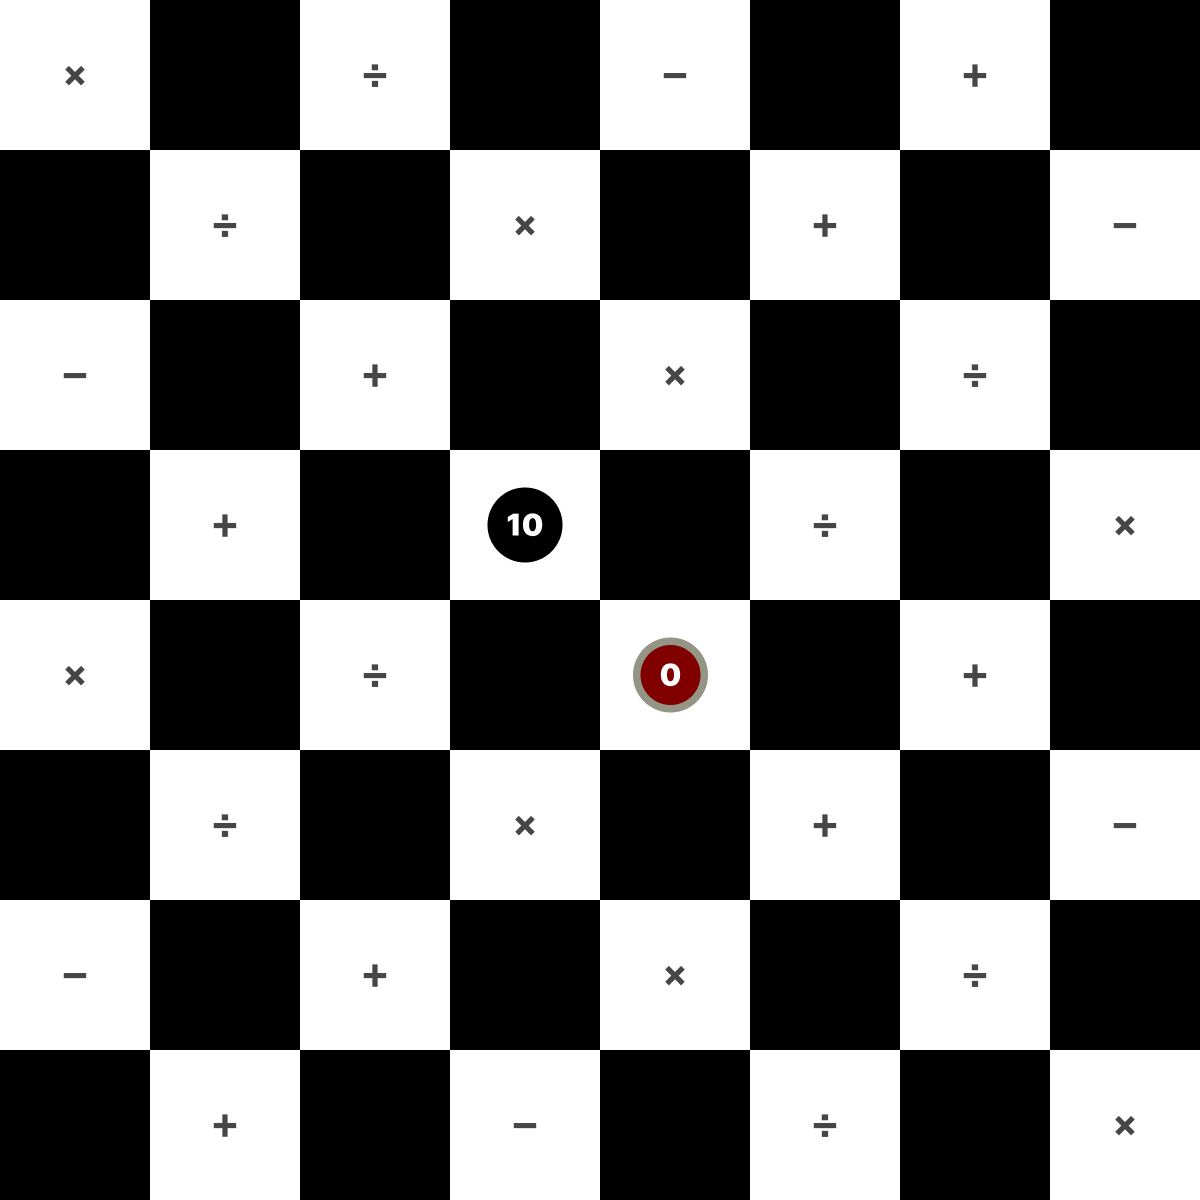
\includegraphics[width=0.4\linewidth]{images/example_state.png}\end{gathered}\right) = \resizebox{0.4\textwidth}{!}{$\begin{bmatrix}
            \gz & \gz & \gz & \gz & \gz & \gz & \gz & \gz & \gz & \gz & \gz & \gz & \gz & \gz & \gz & \gs & \rz & \go & \gz & \gz & \gz & \gz \\
            \gz & \gz & \gz & \gz & \gz & \gz & \gz & \gz & \gz & \gz & \gz & \gz & \gz & \gz & \gz & \gs & \rz & \gz & \go & \gz & \gz & \gz \\
            \gz & \gz & \gz & \gz & \gz & \gz & \gz & \gz & \gz & \gz & \gz & \gz & \gz & \gz & \gz & \gs & \rz & \gz & \gz & \gz & \go & \gz \\
            \gz & \gz & \gz & \gz & \gz & \gz & \gz & \gz & \gz & \gz & \gz & \gz & \gz & \gz & \gz & \gs & \rz & \gz & \gz & \go & \gz & \gz \\
            \gz & \gz & \gz & \gz & \gz & \gz & \gz & \gz & \gz & \gz & \gz & \gz & \gz & \gz & \gz & \gs & \rz & \gz & \go & \gz & \gz & \gz \\
            \gz & \gz & \gz & \gz & \gz & \gz & \gz & \gz & \gz & \gz & \gz & \gz & \gz & \gz & \gz & \gs & \rz & \go & \gz & \gz & \gz & \gz \\
            \gz & \gz & \gz & \gz & \gz & \gz & \gz & \gz & \gz & \gz & \gz & \gz & \gz & \gz & \gz & \gs & \rz & \gz & \gz & \go & \gz & \gz \\
            \gz & \gz & \gz & \gz & \gz & \gz & \gz & \gz & \gz & \gz & \gz & \gz & \gz & \gz & \gz & \gs & \rz & \gz & \gz & \gz & \go & \gz \\
            \gz & \gz & \gz & \gz & \gz & \gz & \gz & \gz & \gz & \gz & \gz & \gz & \gz & \gz & \gz & \gs & \rz & \gz & \gz & \gz & \go & \gz \\
            \gz & \gz & \gz & \gz & \gz & \gz & \gz & \gz & \gz & \gz & \gz & \gz & \gz & \gz & \gz & \gs & \rz & \gz & \gz & \go & \gz & \gz \\
            \gz & \gz & \gz & \gz & \gz & \gz & \gz & \gz & \gz & \gz & \gz & \gz & \gz & \gz & \gz & \gs & \rz & \go & \gz & \gz & \gz & \gz \\
            \gz & \gz & \gz & \gz & \gz & \gz & \gz & \gz & \gz & \gz & \gz & \gz & \gz & \gz & \gz & \gs & \rz & \gz & \go & \gz & \gz & \gz \\
            \gz & \gz & \gz & \gz & \gz & \gz & \gz & \gz & \gz & \gz & \gz & \gz & \gz & \gz & \gz & \gs & \rz & \gz & \gz & \go & \gz & \gz \\
            \gz & \gz & \gz & \gz & \gz & \gz & \gz & \gz & \gz & \gz & \gz & \gz & \gz & \gz & \gz & \gs & \rz & \gz & \gz & \gz & \go & \gz \\
            \gz & \go & \gz & \gz & \gz & \gz & \gz & \gz & \gz & \gz & \gz & \gz & \gz & \go & \go & \gs & \rz & \gz & \go & \gz & \gz & \go \\
            \gz & \gz & \gz & \gz & \gz & \gz & \gz & \gz & \gz & \gz & \gz & \gz & \gz & \gz & \gz & \gs & \rz & \go & \gz & \gz & \gz & \gz \\
            \gz & \gz & \gz & \gz & \gz & \gz & \gz & \gz & \gz & \gz & \gz & \gz & \gz & \gz & \gz & \gs & \rz & \go & \gz & \gz & \gz & \gz \\
            \gz & \gz & \gz & \gz & \gz & \gz & \gz & \gz & \gz & \gz & \gz & \go & \gz & \gz & \gz & \gs & \rz & \gz & \go & \gz & \gz & \gz \\
            \gz & \gz & \gz & \gz & \gz & \gz & \gz & \gz & \gz & \gz & \gz & \gz & \gz & \gz & \gz & \gs & \rz & \gz & \gz & \gz & \go & \gz \\
            \gz & \gz & \gz & \gz & \gz & \gz & \gz & \gz & \gz & \gz & \gz & \gz & \gz & \gz & \gz & \gs & \rz & \gz & \gz & \go & \gz & \gz \\
            \gz & \gz & \gz & \gz & \gz & \gz & \gz & \gz & \gz & \gz & \gz & \gz & \gz & \gz & \gz & \gs & \rz & \gz & \go & \gz & \gz & \gz \\
            \gz & \gz & \gz & \gz & \gz & \gz & \gz & \gz & \gz & \gz & \gz & \gz & \gz & \gz & \gz & \gs & \rz & \go & \gz & \gz & \gz & \gz \\
            \gz & \gz & \gz & \gz & \gz & \gz & \gz & \gz & \gz & \gz & \gz & \gz & \gz & \gz & \gz & \gs & \rz & \gz & \gz & \go & \gz & \gz \\
            \gz & \gz & \gz & \gz & \gz & \gz & \gz & \gz & \gz & \gz & \gz & \gz & \gz & \gz & \gz & \gs & \rz & \gz & \gz & \gz & \go & \gz \\
            \gz & \gz & \gz & \gz & \gz & \gz & \gz & \gz & \gz & \gz & \gz & \gz & \gz & \gz & \gz & \gs & \rz & \gz & \gz & \gz & \go & \gz \\
            \gz & \gz & \gz & \gz & \gz & \gz & \gz & \gz & \gz & \gz & \gz & \gz & \gz & \gz & \gz & \gs & \rz & \gz & \gz & \go & \gz & \gz \\
            \gz & \gz & \gz & \gz & \gz & \gz & \gz & \gz & \gz & \gz & \gz & \gz & \gz & \gz & \gz & \gs & \rz & \go & \gz & \gz & \gz & \gz \\
            \gz & \gz & \gz & \gz & \gz & \gz & \gz & \gz & \gz & \gz & \gz & \gz & \gz & \gz & \gz & \gs & \rz & \gz & \go & \gz & \gz & \gz \\
            \gz & \gz & \gz & \gz & \gz & \gz & \gz & \gz & \gz & \gz & \gz & \gz & \gz & \gz & \gz & \gs & \rz & \gz & \gz & \go & \gz & \gz \\
            \gz & \gz & \gz & \gz & \gz & \gz & \gz & \gz & \gz & \gz & \gz & \gz & \gz & \gz & \gz & \gs & \rz & \gz & \gz & \gz & \go & \gz \\
            \gz & \gz & \gz & \gz & \gz & \gz & \gz & \gz & \gz & \gz & \gz & \gz & \gz & \gz & \gz & \gs & \rz & \gz & \go & \gz & \gz & \gz \\
            \gz & \gz & \gz & \gz & \gz & \gz & \gz & \gz & \gz & \gz & \gz & \gz & \gz & \gz & \gz & \gs & \rz & \go & \gz & \gz & \gz & \gz
        \end{bmatrix}$}
    \end{equation*}
    \caption{Example State Representation with the Draw Count Highlighted}
    \label{fig:example-state-representation-eighteenth}
\end{figure}

The nineteenth to twenty-second column represents the one-hot encoding of the board operator on the current cell as shown as red cells in the example shown in Figure \ref{fig:example-state-representation-nineteenth-twenty-second}. Four dimensions are used to represent one of the four different operators a cell may have. The values of all of these dimensions are zero except for a single dimension that has a value of one if it corresponds to the board operator on the cell.

\begin{figure}[H]
    \begin{equation*} 
        \verb|Encode|\left(\begin{gathered}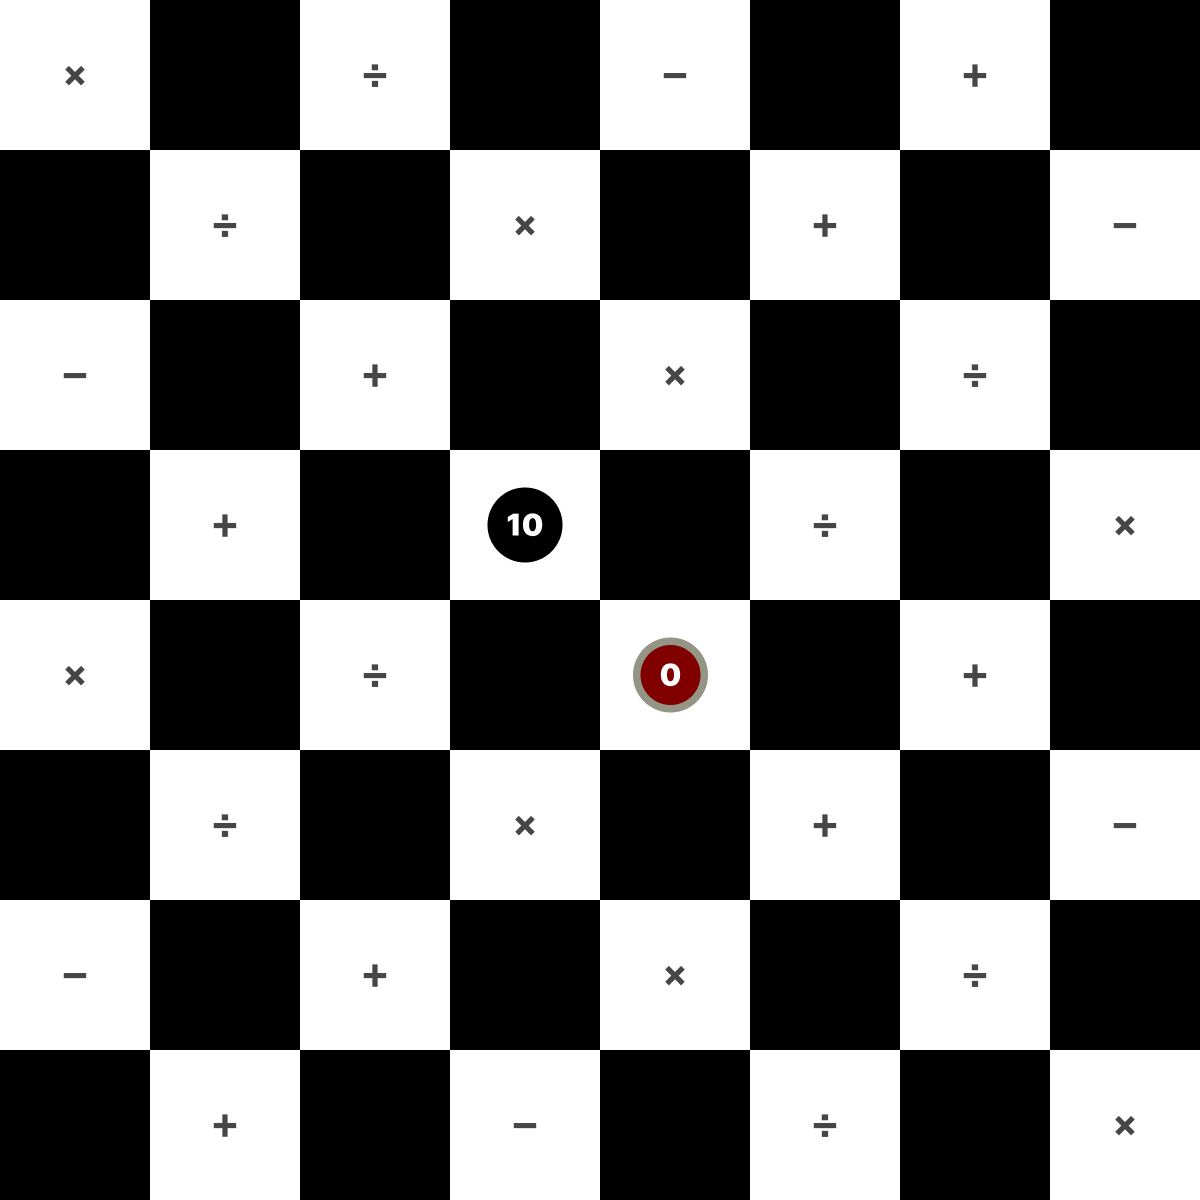
\includegraphics[width=0.4\linewidth]{images/example_state.png}\end{gathered}\right) = \resizebox{0.4\textwidth}{!}{$\begin{bmatrix}
            \gz & \gz & \gz & \gz & \gz & \gz & \gz & \gz & \gz & \gz & \gz & \gz & \gz & \gz & \gz & \gs & \gz & \ro & \rz & \rz & \rz & \gz \\
            \gz & \gz & \gz & \gz & \gz & \gz & \gz & \gz & \gz & \gz & \gz & \gz & \gz & \gz & \gz & \gs & \gz & \rz & \ro & \rz & \rz & \gz \\
            \gz & \gz & \gz & \gz & \gz & \gz & \gz & \gz & \gz & \gz & \gz & \gz & \gz & \gz & \gz & \gs & \gz & \rz & \rz & \rz & \ro & \gz \\
            \gz & \gz & \gz & \gz & \gz & \gz & \gz & \gz & \gz & \gz & \gz & \gz & \gz & \gz & \gz & \gs & \gz & \rz & \rz & \ro & \rz & \gz \\
            \gz & \gz & \gz & \gz & \gz & \gz & \gz & \gz & \gz & \gz & \gz & \gz & \gz & \gz & \gz & \gs & \gz & \rz & \ro & \rz & \rz & \gz \\
            \gz & \gz & \gz & \gz & \gz & \gz & \gz & \gz & \gz & \gz & \gz & \gz & \gz & \gz & \gz & \gs & \gz & \ro & \rz & \rz & \rz & \gz \\
            \gz & \gz & \gz & \gz & \gz & \gz & \gz & \gz & \gz & \gz & \gz & \gz & \gz & \gz & \gz & \gs & \gz & \rz & \rz & \ro & \rz & \gz \\
            \gz & \gz & \gz & \gz & \gz & \gz & \gz & \gz & \gz & \gz & \gz & \gz & \gz & \gz & \gz & \gs & \gz & \rz & \rz & \rz & \ro & \gz \\
            \gz & \gz & \gz & \gz & \gz & \gz & \gz & \gz & \gz & \gz & \gz & \gz & \gz & \gz & \gz & \gs & \gz & \rz & \rz & \rz & \ro & \gz \\
            \gz & \gz & \gz & \gz & \gz & \gz & \gz & \gz & \gz & \gz & \gz & \gz & \gz & \gz & \gz & \gs & \gz & \rz & \rz & \ro & \rz & \gz \\
            \gz & \gz & \gz & \gz & \gz & \gz & \gz & \gz & \gz & \gz & \gz & \gz & \gz & \gz & \gz & \gs & \gz & \ro & \rz & \rz & \rz & \gz \\
            \gz & \gz & \gz & \gz & \gz & \gz & \gz & \gz & \gz & \gz & \gz & \gz & \gz & \gz & \gz & \gs & \gz & \rz & \ro & \rz & \rz & \gz \\
            \gz & \gz & \gz & \gz & \gz & \gz & \gz & \gz & \gz & \gz & \gz & \gz & \gz & \gz & \gz & \gs & \gz & \rz & \rz & \ro & \rz & \gz \\
            \gz & \gz & \gz & \gz & \gz & \gz & \gz & \gz & \gz & \gz & \gz & \gz & \gz & \gz & \gz & \gs & \gz & \rz & \rz & \rz & \ro & \gz \\
            \gz & \go & \gz & \gz & \gz & \gz & \gz & \gz & \gz & \gz & \gz & \gz & \gz & \go & \go & \gs & \gz & \rz & \ro & \rz & \rz & \go \\
            \gz & \gz & \gz & \gz & \gz & \gz & \gz & \gz & \gz & \gz & \gz & \gz & \gz & \gz & \gz & \gs & \gz & \ro & \rz & \rz & \rz & \gz \\
            \gz & \gz & \gz & \gz & \gz & \gz & \gz & \gz & \gz & \gz & \gz & \gz & \gz & \gz & \gz & \gs & \gz & \ro & \rz & \rz & \rz & \gz \\
            \gz & \gz & \gz & \gz & \gz & \gz & \gz & \gz & \gz & \gz & \gz & \go & \gz & \gz & \gz & \gs & \gz & \rz & \ro & \rz & \rz & \gz \\
            \gz & \gz & \gz & \gz & \gz & \gz & \gz & \gz & \gz & \gz & \gz & \gz & \gz & \gz & \gz & \gs & \gz & \rz & \rz & \rz & \ro & \gz \\
            \gz & \gz & \gz & \gz & \gz & \gz & \gz & \gz & \gz & \gz & \gz & \gz & \gz & \gz & \gz & \gs & \gz & \rz & \rz & \ro & \rz & \gz \\
            \gz & \gz & \gz & \gz & \gz & \gz & \gz & \gz & \gz & \gz & \gz & \gz & \gz & \gz & \gz & \gs & \gz & \rz & \ro & \rz & \rz & \gz \\
            \gz & \gz & \gz & \gz & \gz & \gz & \gz & \gz & \gz & \gz & \gz & \gz & \gz & \gz & \gz & \gs & \gz & \ro & \rz & \rz & \rz & \gz \\
            \gz & \gz & \gz & \gz & \gz & \gz & \gz & \gz & \gz & \gz & \gz & \gz & \gz & \gz & \gz & \gs & \gz & \rz & \rz & \ro & \rz & \gz \\
            \gz & \gz & \gz & \gz & \gz & \gz & \gz & \gz & \gz & \gz & \gz & \gz & \gz & \gz & \gz & \gs & \gz & \rz & \rz & \rz & \ro & \gz \\
            \gz & \gz & \gz & \gz & \gz & \gz & \gz & \gz & \gz & \gz & \gz & \gz & \gz & \gz & \gz & \gs & \gz & \rz & \rz & \rz & \ro & \gz \\
            \gz & \gz & \gz & \gz & \gz & \gz & \gz & \gz & \gz & \gz & \gz & \gz & \gz & \gz & \gz & \gs & \gz & \rz & \rz & \ro & \rz & \gz \\
            \gz & \gz & \gz & \gz & \gz & \gz & \gz & \gz & \gz & \gz & \gz & \gz & \gz & \gz & \gz & \gs & \gz & \ro & \rz & \rz & \rz & \gz \\
            \gz & \gz & \gz & \gz & \gz & \gz & \gz & \gz & \gz & \gz & \gz & \gz & \gz & \gz & \gz & \gs & \gz & \rz & \ro & \rz & \rz & \gz \\
            \gz & \gz & \gz & \gz & \gz & \gz & \gz & \gz & \gz & \gz & \gz & \gz & \gz & \gz & \gz & \gs & \gz & \rz & \rz & \ro & \rz & \gz \\
            \gz & \gz & \gz & \gz & \gz & \gz & \gz & \gz & \gz & \gz & \gz & \gz & \gz & \gz & \gz & \gs & \gz & \rz & \rz & \rz & \ro & \gz \\
            \gz & \gz & \gz & \gz & \gz & \gz & \gz & \gz & \gz & \gz & \gz & \gz & \gz & \gz & \gz & \gs & \gz & \rz & \ro & \rz & \rz & \gz \\
            \gz & \gz & \gz & \gz & \gz & \gz & \gz & \gz & \gz & \gz & \gz & \gz & \gz & \gz & \gz & \gs & \gz & \ro & \rz & \rz & \rz & \gz
        \end{bmatrix}$}
    \end{equation*}
    \caption{Example State Representation with the Board Operator Highlighted}
    \label{fig:example-state-representation-nineteenth-twenty-second}
\end{figure}

The twenty-third dimension represents the multiple capture status of the piece in the current cell as shown as red cells in the example shown in Figure \ref{fig:example-state-representation-twenty-third}. The value of this dimension is one if the piece in the current cell is in the middle of a multiple capture and zero if not. This dimension tells whether the piece on the current cell is the only piece that may move for the current game and should continue the multiple capture move.

\begin{figure}[H]
    \begin{equation*} 
        \verb|Encode|\left(\begin{gathered}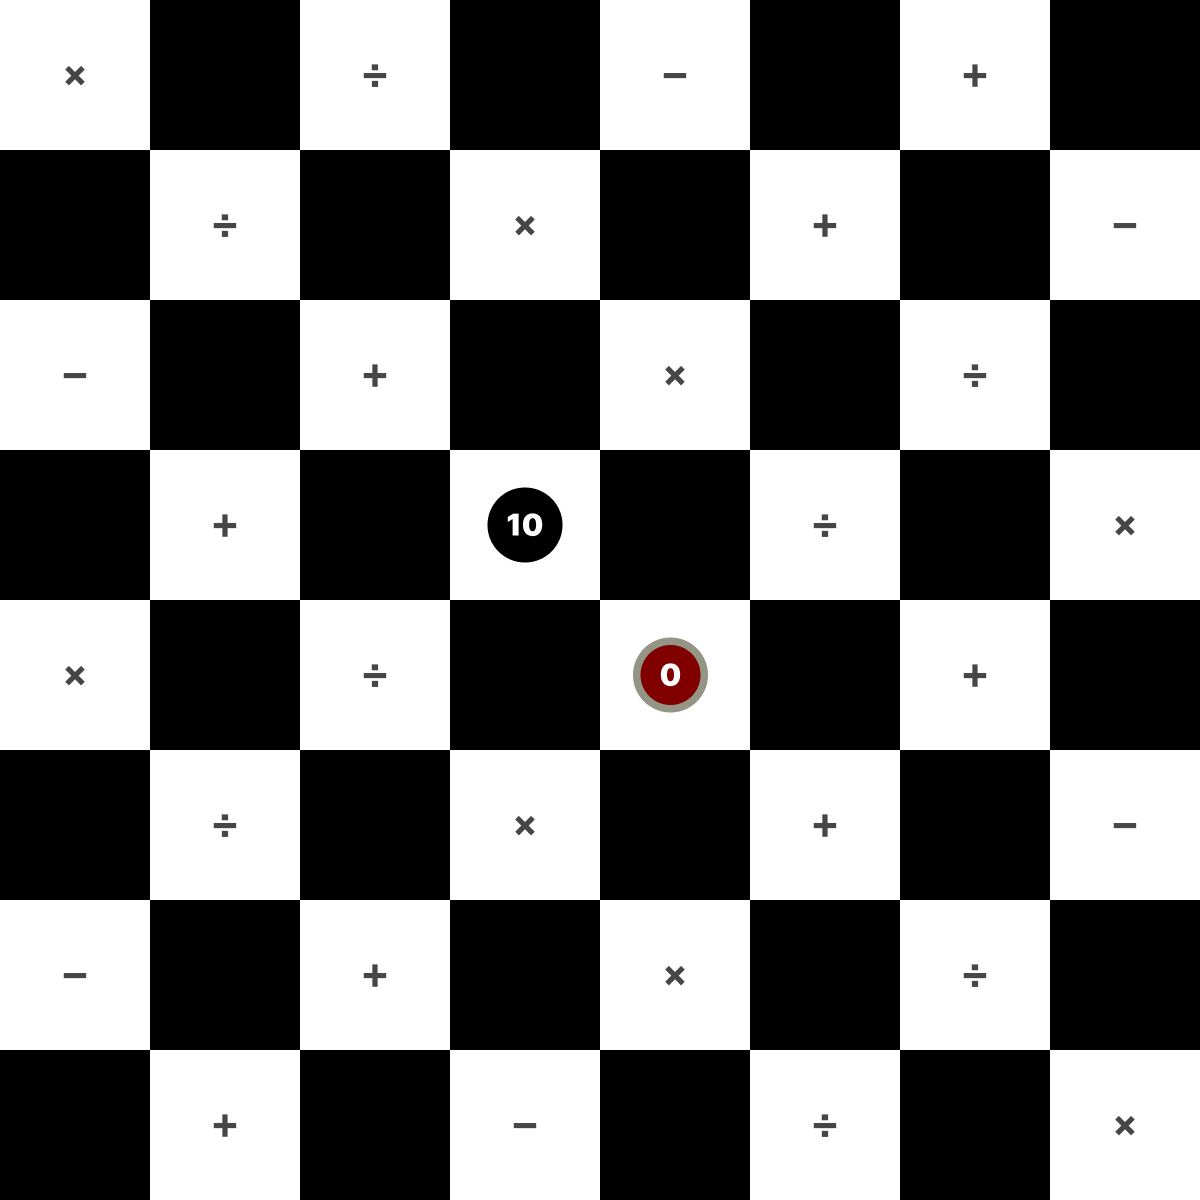
\includegraphics[width=0.4\linewidth]{images/example_state.png}\end{gathered}\right) = \resizebox{0.4\textwidth}{!}{$\begin{bmatrix}
            \gz & \gz & \gz & \gz & \gz & \gz & \gz & \gz & \gz & \gz & \gz & \gz & \gz & \gz & \gz & \gs & \gz & \go & \gz & \gz & \gz & \rz \\
            \gz & \gz & \gz & \gz & \gz & \gz & \gz & \gz & \gz & \gz & \gz & \gz & \gz & \gz & \gz & \gs & \gz & \gz & \go & \gz & \gz & \rz \\
            \gz & \gz & \gz & \gz & \gz & \gz & \gz & \gz & \gz & \gz & \gz & \gz & \gz & \gz & \gz & \gs & \gz & \gz & \gz & \gz & \go & \rz \\
            \gz & \gz & \gz & \gz & \gz & \gz & \gz & \gz & \gz & \gz & \gz & \gz & \gz & \gz & \gz & \gs & \gz & \gz & \gz & \go & \gz & \rz \\
            \gz & \gz & \gz & \gz & \gz & \gz & \gz & \gz & \gz & \gz & \gz & \gz & \gz & \gz & \gz & \gs & \gz & \gz & \go & \gz & \gz & \rz \\
            \gz & \gz & \gz & \gz & \gz & \gz & \gz & \gz & \gz & \gz & \gz & \gz & \gz & \gz & \gz & \gs & \gz & \go & \gz & \gz & \gz & \rz \\
            \gz & \gz & \gz & \gz & \gz & \gz & \gz & \gz & \gz & \gz & \gz & \gz & \gz & \gz & \gz & \gs & \gz & \gz & \gz & \go & \gz & \rz \\
            \gz & \gz & \gz & \gz & \gz & \gz & \gz & \gz & \gz & \gz & \gz & \gz & \gz & \gz & \gz & \gs & \gz & \gz & \gz & \gz & \go & \rz \\
            \gz & \gz & \gz & \gz & \gz & \gz & \gz & \gz & \gz & \gz & \gz & \gz & \gz & \gz & \gz & \gs & \gz & \gz & \gz & \gz & \go & \rz \\
            \gz & \gz & \gz & \gz & \gz & \gz & \gz & \gz & \gz & \gz & \gz & \gz & \gz & \gz & \gz & \gs & \gz & \gz & \gz & \go & \gz & \rz \\
            \gz & \gz & \gz & \gz & \gz & \gz & \gz & \gz & \gz & \gz & \gz & \gz & \gz & \gz & \gz & \gs & \gz & \go & \gz & \gz & \gz & \rz \\
            \gz & \gz & \gz & \gz & \gz & \gz & \gz & \gz & \gz & \gz & \gz & \gz & \gz & \gz & \gz & \gs & \gz & \gz & \go & \gz & \gz & \rz \\
            \gz & \gz & \gz & \gz & \gz & \gz & \gz & \gz & \gz & \gz & \gz & \gz & \gz & \gz & \gz & \gs & \gz & \gz & \gz & \go & \gz & \rz \\
            \gz & \gz & \gz & \gz & \gz & \gz & \gz & \gz & \gz & \gz & \gz & \gz & \gz & \gz & \gz & \gs & \gz & \gz & \gz & \gz & \go & \rz \\
            \gz & \go & \gz & \gz & \gz & \gz & \gz & \gz & \gz & \gz & \gz & \gz & \gz & \go & \go & \gs & \gz & \gz & \go & \gz & \gz & \ro \\
            \gz & \gz & \gz & \gz & \gz & \gz & \gz & \gz & \gz & \gz & \gz & \gz & \gz & \gz & \gz & \gs & \gz & \go & \gz & \gz & \gz & \rz \\
            \gz & \gz & \gz & \gz & \gz & \gz & \gz & \gz & \gz & \gz & \gz & \gz & \gz & \gz & \gz & \gs & \gz & \go & \gz & \gz & \gz & \rz \\
            \gz & \gz & \gz & \gz & \gz & \gz & \gz & \gz & \gz & \gz & \gz & \go & \gz & \gz & \gz & \gs & \gz & \gz & \go & \gz & \gz & \rz \\
            \gz & \gz & \gz & \gz & \gz & \gz & \gz & \gz & \gz & \gz & \gz & \gz & \gz & \gz & \gz & \gs & \gz & \gz & \gz & \gz & \go & \rz \\
            \gz & \gz & \gz & \gz & \gz & \gz & \gz & \gz & \gz & \gz & \gz & \gz & \gz & \gz & \gz & \gs & \gz & \gz & \gz & \go & \gz & \rz \\
            \gz & \gz & \gz & \gz & \gz & \gz & \gz & \gz & \gz & \gz & \gz & \gz & \gz & \gz & \gz & \gs & \gz & \gz & \go & \gz & \gz & \rz \\
            \gz & \gz & \gz & \gz & \gz & \gz & \gz & \gz & \gz & \gz & \gz & \gz & \gz & \gz & \gz & \gs & \gz & \go & \gz & \gz & \gz & \rz \\
            \gz & \gz & \gz & \gz & \gz & \gz & \gz & \gz & \gz & \gz & \gz & \gz & \gz & \gz & \gz & \gs & \gz & \gz & \gz & \go & \gz & \rz \\
            \gz & \gz & \gz & \gz & \gz & \gz & \gz & \gz & \gz & \gz & \gz & \gz & \gz & \gz & \gz & \gs & \gz & \gz & \gz & \gz & \go & \rz \\
            \gz & \gz & \gz & \gz & \gz & \gz & \gz & \gz & \gz & \gz & \gz & \gz & \gz & \gz & \gz & \gs & \gz & \gz & \gz & \gz & \go & \rz \\
            \gz & \gz & \gz & \gz & \gz & \gz & \gz & \gz & \gz & \gz & \gz & \gz & \gz & \gz & \gz & \gs & \gz & \gz & \gz & \go & \gz & \rz \\
            \gz & \gz & \gz & \gz & \gz & \gz & \gz & \gz & \gz & \gz & \gz & \gz & \gz & \gz & \gz & \gs & \gz & \go & \gz & \gz & \gz & \rz \\
            \gz & \gz & \gz & \gz & \gz & \gz & \gz & \gz & \gz & \gz & \gz & \gz & \gz & \gz & \gz & \gs & \gz & \gz & \go & \gz & \gz & \rz \\
            \gz & \gz & \gz & \gz & \gz & \gz & \gz & \gz & \gz & \gz & \gz & \gz & \gz & \gz & \gz & \gs & \gz & \gz & \gz & \go & \gz & \rz \\
            \gz & \gz & \gz & \gz & \gz & \gz & \gz & \gz & \gz & \gz & \gz & \gz & \gz & \gz & \gz & \gs & \gz & \gz & \gz & \gz & \go & \rz \\
            \gz & \gz & \gz & \gz & \gz & \gz & \gz & \gz & \gz & \gz & \gz & \gz & \gz & \gz & \gz & \gs & \gz & \gz & \go & \gz & \gz & \rz \\
            \gz & \gz & \gz & \gz & \gz & \gz & \gz & \gz & \gz & \gz & \gz & \gz & \gz & \gz & \gz & \gs & \gz & \go & \gz & \gz & \gz & \rz
        \end{bmatrix}$}
    \end{equation*}
    \caption{Example State Representation with the Multiple Capture Status Highlighted}
    \label{fig:example-state-representation-twenty-third}
\end{figure}

\section{Action Representation}

The action is a scalar value represented as an index to the action set of Damath. The action set of Damath can be represented as a Cartesian product of the set of board positions, the set of four cardinal directions to which a Damath piece can take, and the set of seven distances that a Damath piece can cover as shown in Figure \ref{fig:action-set-damath}.

\begin{figure}[H]
    \centering
    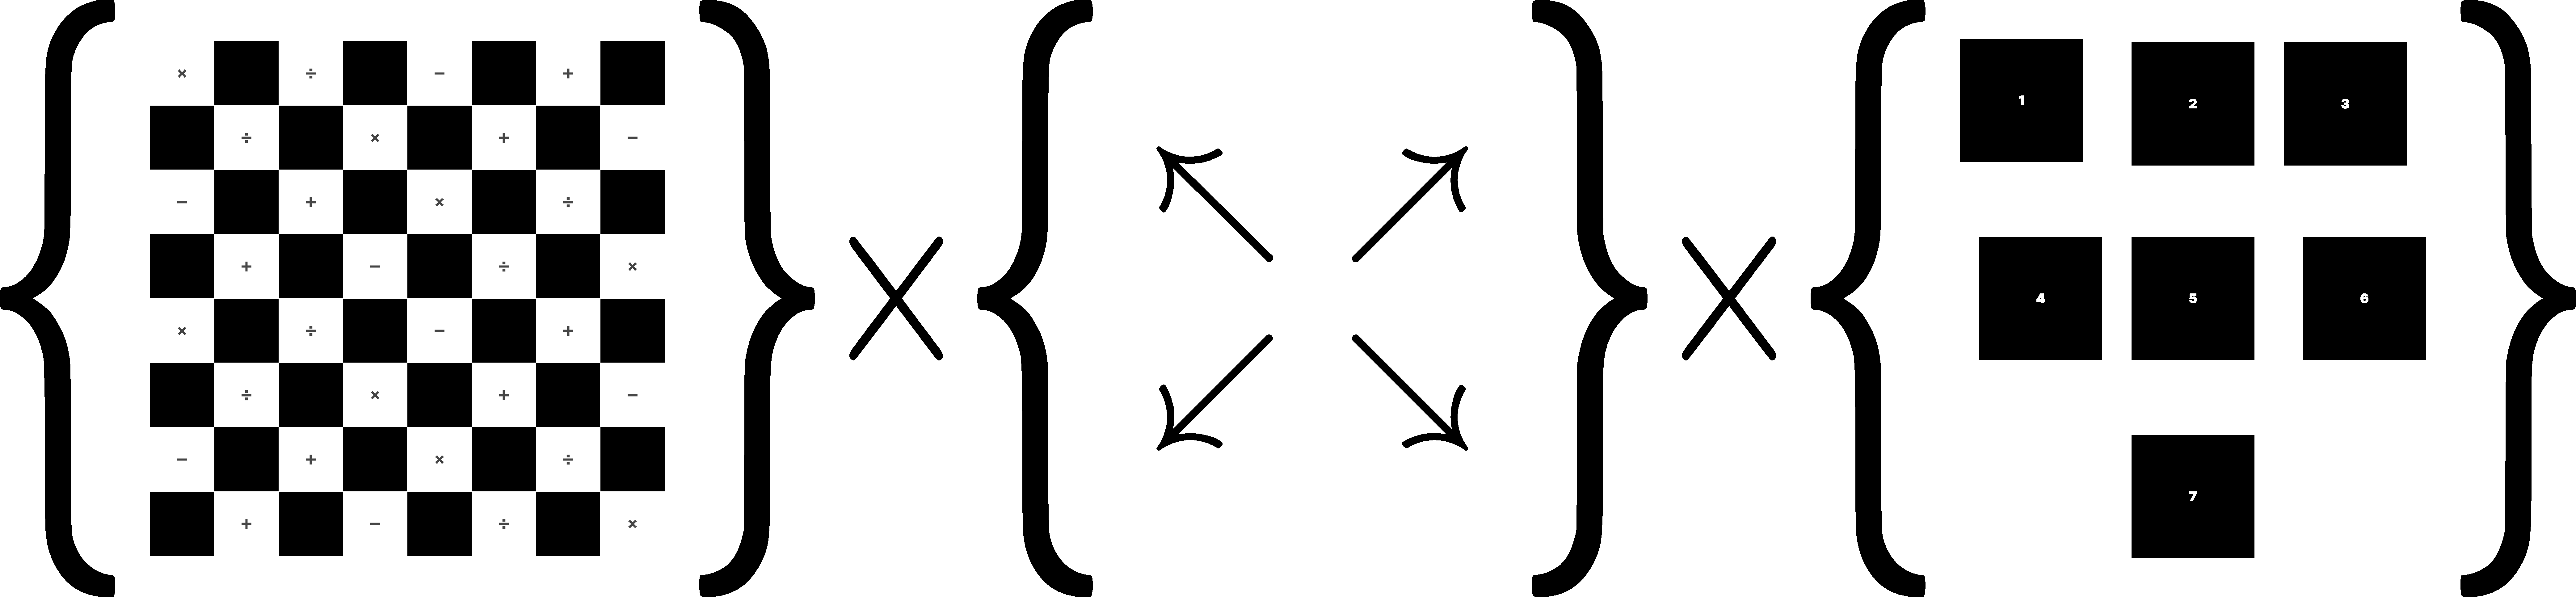
\includegraphics[width=0.7\linewidth]{images/Action Space.pdf}
    \caption{Action Set of Damath}
    \label{fig:action-set-damath}
\end{figure}

The action set of Damath is a $8 \times 8 \times 4 \times 7$ matrix with each of the $4 \times 7$ planes corresponding to an $8 \times 8$ matrix containing pieces at specific board positions that can perform a specific combination of the four directions and seven distances. The values of these matrices are all zero except for cells that contain a piece of the current player that may make a legal move in the direction and distance specified by one of the $4 \times 7$ planes.

The set of four cardinal directions to which a Damath piece can take contains the up-left direction, the up-right direction, the down-left direction, and the down-right direction. A normal piece can only appear on the two up-direction planes if it is owned by the red player, and the two down-direction planes if it is owned by the black player. A dama piece can appear on all four direction planes.

The set of seven distances a Damath piece can cover contains distances from one to seven units. A normal piece can only appear on one-unit distance planes for valid jump moves and two-unit distance planes for valid capture moves. A dama piece can appear on all seven distance planes for valid capture and jump moves. 

The position of the piece, the direction it takes and the distance it covers can be derived from a given action $a$ by using the functions shown in Equation \ref{eq:action-formula}.
\begin{align} 
    \begin{split}
        \text{position}_x(a) &= (a \bmod (8 * 8 * 4)) \bmod (8 * 8)) \bmod 8 \\
        \text{position}_y(a) &= \left\lfloor \frac{(a \bmod (8 * 8 * 4)) \bmod (8 * 8)}{8} \right\rfloor\\
        \text{distance}(a) &= \left\lfloor \frac{a}{8 * 8 * 4}\right\rfloor + 1 \\
        \text{direction}(a) &= 
        \begin{cases}
            \text{top left}, & \left\lfloor \frac{a \bmod (8 * 8 * 4))}{8 * 8} \right\rfloor = 0 \\
            \text{top right}, & \left\lfloor \frac{a \bmod (8 * 8 * 4))}{8 * 8} \right\rfloor = 1\\
            \text{bottom left}, & \left\lfloor \frac{a \bmod (8 * 8 * 4))}{8 * 8} \right\rfloor = 2\\
            \text{bottom right}, & \left\lfloor \frac{a \bmod (8 * 8 * 4))}{8 * 8} \right\rfloor = 3\\
        \end{cases}
    \end{split}
    \label{eq:action-formula}
\end{align}

\section{Model Architecture}

The neural network $f_{\theta}$ in the original AlphaZero paper by \cite{silver2017masteringchessshogiselfplay} takes an input state $s$ and produces a tuple $f_{\theta}(s) = (p, v)$ where $p$ is the policy vector which contains all the probabilities of all actions defined by the action space, and $v \in [-1, 1]$ is the value scalar that estimates the expected outcome of the current state of the game $s$. The input state $s$ used in this study is obtained by getting the encoded state of the current state of the game. The policy vector $p$ is masked against the legal actions of the current game before being used by the MCTS algorithm to prevent the model from assigning probabilities to illegal actions. The value scalar $v$ estimates that the outcome of the game is a loss when it is close to $-1$, a draw when it is close to zero and a win when it is close to $1$.

% ADVISER COMMENT (DON'T DELETE): change "paper" to either study, research, or work
This study replaced the value scalar with a three-dimensional win-draw-loss (WDL) vector $v_{\text{WDL}} = (p_w, p_d, p_l)$ inspired by \cite{czech2024representationmattersmasteringchess} where $v_{\text{WDL}}$ is the WDL vector, $p_w$ is the probability of winning, $p_d$ is the probability of having a draw, and $p_l$ is the probability of losing with $p_w + p_d + p_l = 1$. This representation provides the model with richer outcome information, allowing it to explicitly differentiate between winning, drawing, and losing probabilities rather than collapsing this information into a single scalar value. The MCTS implementation still requires a scalar value for backpropagation that is computed by $v = p_w - p_l$.

According to \cite{dosovitskiy2021imageworth16x16words}, recent developments in the field of computer vision have shown that vision transformers are capable of beating Convolutional Neural Networks in image recognition tasks. This paper replaces the model architecture used by \cite{Popic_Boskovic_Brest_2021} from a deep Convolutional Neural Network architecture to a Vision Transformer with a jumbo CLS token architecture. The vision transformer with a jumbo CLS token model architecture would be used to infer the WDL probabilities and the action priors of a state of a game. A summary of all the values used for the model architecture is shown in Table \ref{tab:model-configuration-summary}.

\begin{table}[H]
  \centering
  \begin{tabular}{llp{7.5cm}}
    \hline 
    Configuration              & Value & Description                                                         \\ \hline
    \verb|embedding_dim|       & 256   & The embedding dimension of a piece.                                 \\
    \verb|num_cls_tokens|      & 8     & The size of the jumbo CLS tokens.                                   \\
    \verb|num_blocks|          & 16    & The number of transformer encoder blocks.                           \\
    \verb|num_attention_heads| & 16    & The  number of attention heads of each multi-head attention layers. \\
    \verb|mlp_hidden_size|     & 512   & The hidden size of the linear layer of the multilayer perceptron.   \\
    \verb|mlp_dropout_ratio|   & 0.1   & The dropout ratio of the multilayer perceptron.                     \\ \hline
  \end{tabular}
  \caption{Summary of All of the Values Used for the Model Architecture}
  \label{tab:model-configuration-summary}
\end{table}

The architecture shown in Figure \ref{fig:jumbo-vit} takes the $32 \times 23$ matrix representation of the current state of the game as input to the model. The input then passes to an embedding layer that outputs a jumbo CLS token and the input embedding concatenated together. The jumbo CLS token and input embedding concatenated together then passes to a transformer encoder. After passing through the transformer encoder, the output of the jumbo CLS token is flattened and passed to the WDL and Policy head of the model.

\begin{figure}[H]
    \centering
    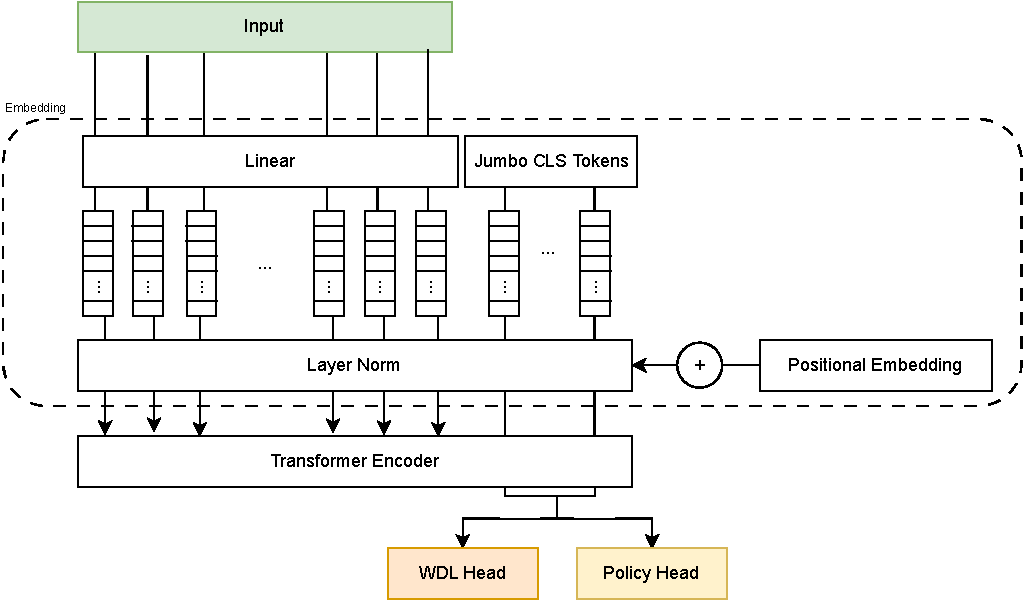
\includegraphics[width=\linewidth]{images/JumboViT.pdf}
    \caption{Overview of the Model Architecture}
    \label{fig:jumbo-vit}
\end{figure}

% ADVISER COMMENT (DON'T DELETE): need to define what the variable represent and what the values are
% ADVISER COMMENT (DON'T DELETE,2025-05-30): still need to define what the variables represent and if possible what the values are. EX: what is "num_cls_tokens"? what does it represent? what is the value used for this?

% RESEARCHER'S REPLY (2025-05-31): we added a new section to the preliminaries explaining the various parts of a vision transformer. each variable shown in the table has description matching those that are found in the preliminary. additionally, we also added explanation to each variables every time they show up in the methodology.

The input to the embedding layer used in the model first passes to a linear layer with a $23 \times \verb|embedding_dim|$ weight matrix and the output of this layer is the input embedding. The \verb|embedding_dim| is the number of dimensions of the embedding vector of a cell. Each dimension of the embedding vector encodes a learned feature of the cell that the model learns during the training phase. These learned features are the model's understanding of a specific cell in the board. An example of a feature of a cell that the model might learn is the specific numeric value of the piece that the cell currently contains.

% The internal representation of the state used by the model is the embedding vector obtained by applying the embedding layer to the encoded game state. By increasing the number of \verb|embedding_dim|, the model will be able to encode and learn more information about the cell and its features. This learned embedding captures the semantic meaning of each cell's state in a format optimized for the transformer's attention mechanisms to process spatial and strategic relationships across the Damath board.

The researchers prepend multiple learnable embeddings to the input embedding before passing through a layer normalization layer. These learnable embeddings concatenated into a single vector is the jumbo CLS token with a width of $\verb|num_cls_tokens|$. The jumbo CLS token carries all the necessary global information from the entire sequence of board cells. A $\verb|num_cls_tokens| + 32 \times \verb|embedding_dim|$ learnable positional embedding is added to the input embedding to retain positional information.

The transformer encoder used in the model architecture as shown in Figure \ref{fig:transformer-encoder} is made up of \verb|num_blocks| blocks followed by a layer normalization layer. The variable \verb|num_blocks| denotes the number of blocks as defined in Figure \ref{fig:transformer-encoder}, it also controls how deep the model is. A deeper model would let the model think and learn more about the game at the expense of longer training time.

\begin{figure}[H]
    \centering
    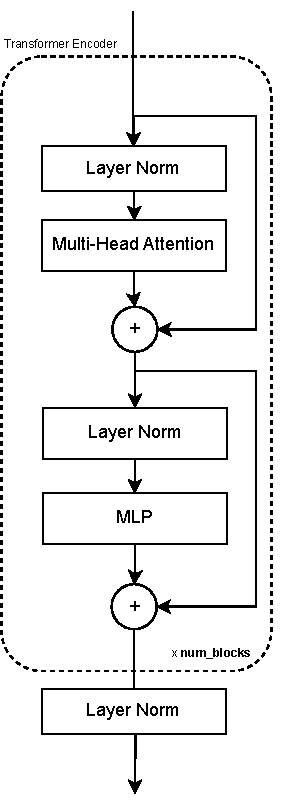
\includegraphics[width=0.2\linewidth]{images/TransformerEncoder.pdf}
    \caption{Transformer Encoder of the Model Architecture}
    \label{fig:transformer-encoder}
\end{figure}

The input to a transformer encoder block is first stored in a residual layer. The input then passes to a layer normalization layer. The output then passes to a multi-head attention layer with \verb|num_attention_heads| heads. This variable indicates the number of attention heads as defined in Equation \ref{eq:single-head}. The residual layer is added back to the output. The output is stored in a new residual layer. The output then passes through another layer normalization layer. The output then passes through a multilayer perceptron. The residual layer is added back to the output. 

The multilayer perceptron layer (MLP) used inside a transformer encoder block is shown in Figure \ref{fig:encoder-mlp}. The input to the MLP first passes through a linear layer with a weight matrix $\verb|embedding_dim| \times \verb|mlp_hidden_size|$. The Gaussian linear error units function is then applied to the output. The output is then passed to another linear layer with a $\verb|mlp_hidden_size| \times \verb|embedding_dim|$ weight matrix. The \verb|mlp_hidden_size| indicates the dimension of the hidden layer as defined in Figure \ref{fig:original-vit}.

The output then finally passes to a dropout layer with a \verb|mlp_dropout_prob| probability of an element to be zeroed. The dropout layer turns off some parameters of the model by turning them into zero based on the \verb|mlp_dropout_prob| probability. This reduces the overfitting of the model, where it performs well on training data but fails massively on new data. This prevents backpropagation of the loss in the zeroed parameters, forcing other parameters of the layer to assume more or less responsibility by taking a probabilistic approach. 

\begin{figure}[H]
    \centering
    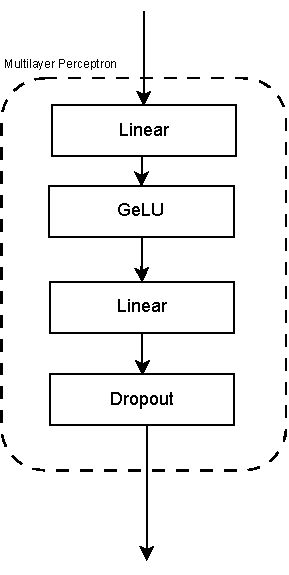
\includegraphics[width=0.2\linewidth]{images/MLP.pdf}
    \caption{Multilayer Perceptron of the Transformer Encoder Block}
    \label{fig:encoder-mlp}
\end{figure}

The WDL head shown in Figure \ref{fig:wdl-head} first passes the flattened output of the jumbo CLS tokens through a linear layer with a weight matrix of size $\verb|num_cls_tokens| \times \verb|embedding_dim| \times 3$ followed by a \verb|softmax| layer. The policy head shown in Figure \ref{fig:policy-head} just passes the flattened output of the jumbo CLS tokens through a linear layer with a weight matrix of size $\verb|num_cls_tokens| \times \verb|embedding_dim| \times 8 \times 8 \times  4 \times 7$.

\begin{figure}[H]
    \centering
    \begin{subfigure}{0.4\linewidth}
        \centering
        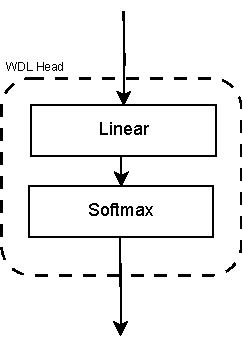
\includegraphics[width=0.3\linewidth]{images/WDLHead.pdf}
        \caption{WDL Head}
        \label{fig:wdl-head}
    \end{subfigure}
    \quad
    \begin{subfigure}{0.4\linewidth}
        \centering
        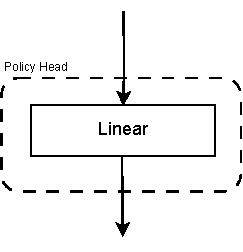
\includegraphics[width=0.5\linewidth]{images/PolicyHead.pdf}
        \caption{Policy Head}
        \label{fig:policy-head}
    \end{subfigure}
    \caption{Output Heads of the Model Architecture}
    \label{fig:model-output}
\end{figure}

\section{Model Generation}

The ultimate goal of the paper is to produce a model that can beat human players in the game of Damath, it has three phases the self-play data generation, model training and model evaluation. These three phases are repeated \verb|num_iterations| times, with each iteration producing a better model. A summary of all the parameters used in model generation is shown in Table \ref{tab:configuration-summary}.

\begin{table}[htb]
  \centering
  \begin{tabular}{llp{7.5cm}}
    \hline 
    Parameter                         & Value              & Description                                                                  \\ \hline
    \verb|num_iterations|             & 20                 & The number of learning iterations.                                           \\
    \verb|num_self_play_games|        & $5000$             & The number of self-play games per learning iteration.                         \\
    \verb|num_self_play_simulations|  & 100                & The number of MCTS simulations performed for each move for game during the self-play data generation phase.           \\
    \verb|num_training_epochs|        & 10                 & The number of training epochs. This refers to the number of size the model is exposed through the whole dataset made throughout the self-play data generation phase.                                              \\
    \verb|num_evaluation_games|       & 100                & The number of games for evaluating the best model against the current model. \\
    \verb|num_evaluation_simulations| & 100                & The number of simulations made for each rounds of evaluation.                \\
    \verb|learning_rate|              & $1 \times 10^{-3}$ & The learning rate used for training the model. The learning rate controls the step size made by the optimizer during its training phase.  \\
    \verb|batch_size|                 & 1024               & The batch size used for training.                                            \\
    \verb|temperature|                & 1.25               & The temperature value used in self play.                                     \\ \hline
  \end{tabular}
  \caption{Summary of All of the Parameters Used in Model Generation}
  \label{tab:configuration-summary}
\end{table}

The pseudocode shown in Algorithm \ref{alg:model-generation} summarizes the entire process. 
The algorithm first initializes a model with random parameters. The current best model is cloned from this model. The dataset composed of $(p, v, s)$ is then generated through self-play where $s$ is state of the game, $p$ is the policy vector, and $v$ is the value vector.

\begin{algorithm}[H]
    \begin{algorithmic}[1]
        \Function{learn}{}
          \State model $\gets$ initialize with random parameters
          \State best\_model $\gets$ \Call{clone}{model}
          \Repeat
            \State dataset $\gets$ \Call{self\_play}{best\_model}
            \State \Call{train}{model, dataset}
            \State wins, draws, losses $\gets$ \Call{evaluate}{model, best\_model}
            \If{$\text{wins} + \text{draws} \ge 0.6 \times \text{num\_evaluations\_games}$} 
                \State best\_model $\gets$ \Call{clone}{model}
            \EndIf
            \Until{$n = \text{num\_iterations}$}
           \State \Return best\_model
        \EndFunction
    \end{algorithmic}
    \caption{Pseudocode for the Model Generation}
    \label{alg:model-generation}
\end{algorithm}

The model is then trained from this dataset. After the training phase, the model is then evaluated by pitting it against the best model. If the wins and draws of the model exceeds $60\%$ of the total number of evaluations, the current model is then assigned as the best model. This process is repeated \verb|num_iterations| times.

% ADVISER COMMENT (DON'T DELETE): need to add also the list of software and/or programs used and what versions were used
The researchers used C++23 and LibTorch 2.7 for the model generation algorithm shown in Algorithm \ref{alg:model-generation}.  The model generation is ran on the cloud using \cite{vastai} % ADVISER COMMENT (DON'T DELETE,2025-05-30): need to cite website/service
with a computer that has 515673MiB of RAM, an AMD Ryzen Threadripper PRO 3975WX CPU with 32-Cores at 3.5000 GHz clock speed, and an NVIDIA GeForce RTX 4090 GPU on an Ubuntu 25.04 Linux Virtual Machine.

\subsection{Self-Play Data Generation}

The dataset needed for training the model is produced by pitting the best model against itself. The self-play data generation as shown in Algorithm \ref{alg:data-generation} starts with assigning $s$ to the initial state of the game, and while $s$ is not a terminal state, it calls the Monte-Carlo Tree Search procedure outlined in Algorithm \ref{alg:mcts}, to produce a policy vector $p$ which contains the probabilities of each action that the model should take in that state $s$. The tuple $(s, p)$ is then recorded, the action is produced by sampling from $p^{1/\verb|temperature|}$. 

\begin{algorithm}[H]
    \begin{algorithmic}[1]
        \Function{self\_play}{model}
            \State dataset $\gets$ \{\}
            \Repeat
            \State history $\gets$ \{\}
            \State $s$ $\gets$ game.initial\_state()
            \Loop
                \State $p$ $\gets$ \Call{search}{$s$, model}
                \State history $\gets$ history $\cup$ ($s$, $p$)
                \State action $\gets$ \Call{sample\_distribution}{$p^{1/\text{temperature}}$}
                \State $s'$ $\gets$ game.apply\_action($s$, action)
                \If{$s'$ is terminal}
                    \ForAll{($s_i$, $p_i$) $\in$ history}
                        \State outcome $\gets$ game.get\_outcome($s'$, action)

                        \If{$s_i$ and $s$ have different players}
                          \State flip outcome
                        \EndIf

                        \If{outcome is win}
                          \State $v_i$ $\gets$ $[1, 0, 0]$
                        \ElsIf{outcome is lose}
                          \State $v_i$ $\gets$ $[0, 0, 1]$
                        \ElsIf{outcome is draw}
                          \State $v_i$ $\gets$ $[0, 1, 0]$
                        \EndIf
                        \State dataset $\gets$ dataset $\cup$ ($p_i$, $v_i$, $s_i$)
                    \EndFor
                    \State \textbf{break}
                \EndIf
                \State $s$ $\gets$ $s'$
            \EndLoop
            \Until{$n = \text{num\_self\_play\_games}$}
        \State \Return{dataset}
        \EndFunction
    \end{algorithmic}
    \caption{Pseudocode for the Self-Play Data Generation Phase of the AlphaZero Framework}
    \label{alg:data-generation}
\end{algorithm}

By raising the each element of $p$ by $1/\verb|temperature|$, the model is encouraged to explore actions that have low-probability. The next state $s'$ is then derived from applying the action to the state $s$. 

If $s'$ is not a terminal state the previous state $s$ is assigned to $s'$, otherwise if $s'$ is a terminal state, then the algorithm loops through all the tuples $(s_i, p_i) \in \text{history}$, if $s_i$ and the previous state $s$ have different players the perspective of the outcome is flipped, and the value $v_i$ is recorded as the one-hot encoding of the outcome. Finally, the tuple $(p_i, v_i, s_i)$ is appended to the dataset. After all the elements in \verb|history| are looped then the inner loop is terminated. This process is repeated for \verb|num_self_play_games| times.

The MCTS Algorithm guides the model in making actions. It has three phases, the selection, expansion, and backpropagation as shown in Algorithm \ref{alg:mcts}.

\begin{algorithm}[H]
    \begin{algorithmic}[1]
        \Function{search}{$s$, model, simulations}
            \State root $\gets$ Node($s$)
            \Repeat
                \State node $\gets$ root
                \State $s'$, node $\gets$ \Call{select}{node}
                \If{$s'$ is terminal}
                    \If{$s$ and $s'$ have different players}
                      \State flip outcome
                    \EndIf
                    \If{outcome is win}
                      \State $v$ $\gets$ $1$
                    \ElsIf{outcome is draw}
                      \State $v$ $\gets$ $0$
                    \ElsIf{outcome is loss}
                      \State $v$ $\gets$ $-1$
                    \EndIf
                \Else
                    \State $v$ $\gets$ \Call{expand}{s, model}
                \EndIf
        
                \State \Call{backpropagate}{node, $v$}
            \Until{$n = \text{simulations}$}

            \State $p \gets \{\}$
            \ForAll{child $\in$ root.children}
            \State $p \gets p \cup \text{child.visits}$
            \EndFor
            \State \Return $p / \sum p$
        \EndFunction
    \end{algorithmic}
    \caption{Monte-Carlo Tree Search Algorithm}
    \label{alg:mcts}
\end{algorithm}

The selection phase selects the node with the highest score as shown in Algorithm \ref{alg:select}. The score function takes into account the perspective of the player who played the previous move. If the previous player is not equal to the current player we adjust the score to select the action that minimizes the score of the player otherwise it selects the action that maximizes the score. 

\begin{algorithm}[H]
    \begin{algorithmic}[1]
        \Function{select}{$s$, node}
            \While{node.is\_expanded()}
                \State node $\gets$ \Call{select\_child}{node}
                \State $s$ $\gets$ game.apply\_action($s$, node.action)
            \EndWhile
            \State \Return $s$, node
        \EndFunction
        
        \Function{select\_child}{node}
            \State child\_scores $\gets$ \{\}
            \ForAll{child $\in$ node.children}
                \State child\_scores $\gets$ child\_scores $\cup$ \Call{score}{child}
            \EndFor
            \Return \Call{max}{child\_scores}
        \EndFunction
        
        \Function{score}{node}
            \If{node.visits $>$ 0}
                \State mean $\gets \dfrac{1}{2}\cdot\left(\dfrac{ \text{node.value} }{ \text{node.visits} } + 1\right)$
                \If{node.parent.player $\neq$ node.player}
                    \State mean $\gets$ 1 $-$ mean
                \EndIf
            \Else
                \State mean $\gets$ 0
            \EndIf
            \State \Return $\text{mean} + \text{node.prior} \cdot C \cdot \dfrac{\sqrt{\text{node.parent.visits}}}{1 + \text{node.visits}}$  
        \EndFunction
    \end{algorithmic}
    \caption{Select Function for the Monte-Carlo Tree Search Algorithm}
    \label{alg:select}
\end{algorithm}

The algorithm repeats the selection phase until it encounters a node that is not expanded. There are two cases, it encounters terminal node or a non-terminal node. 

If it encounters a non-terminal node, then this signifies an action that has not been explored yet and the node is expanded by using the Algorithm shown in \ref{alg:expand}. The canonical MCTS uses a rollout phase that randomly selects an action from the legal actions. Similar to the paper by \cite{silver2017masteringchessshogiselfplay}, we use the model to evaluate the possible actions and assign a probability to each of them. To restrict the model from assigning probabilities to invalid actions, this algorithm obtains the legal actions from the game and filters the policy vector for only the legal actions.

\begin{algorithm}[H]
    \begin{algorithmic}[1]
        \Function{expand}{$s$, model}
            \State $\text{legal\_actions} \gets \text{game.get\_legal\_actions(s)}$
            \State $p, v \gets \text{model(s)}$
            \State $p \gets \Call{softmax}{p}$
            \State $p \gets \Call{filter}{\text{legal\_actions}, p}$
            \State $p \gets p / \sum p$
        
            \For{(action, prior) $\in$ (legal\_actions, policy)}
                \State $s' \gets \text{game.apply\_action($s$, action)}$
                \State parent.children $\gets$ parent.children $\cup$ Node($s'$, action, prior)
            \EndFor
            \State $(p_w, p_d, p_l) \gets v$ 
            \State \Return $p_w - p_l$
        \EndFunction
    \end{algorithmic}
    \caption{Expand Function for the Monte-Carlo Tree Search Algorithm}
    \label{alg:expand}
\end{algorithm}

If it encounters a terminal node, then it backpropagates the outcome of the game as shown in Algorithm \ref{alg:backpropagate}. The backpropagated value is a scalar value $\in [-1, 1]$ which is $1$ for win, $-1$ for lose and $0$ for draw. The backpropagation phase is essential for updating the statistics of the nodes that have been traversed by the current iteration. Here, it updates the cumulative value of each node as well as their respective visit counts.

\begin{algorithm}[H]
    \begin{algorithmic}[1]
        \Function{backpropagate}{node, value}
            \While{node $\neq$ null}
                \State node.visits += 1
                \If{node.parent.state.player == node.state.player} 
                    \State node.value += value
                \Else
                    \State node.value -= value
                \EndIf
                \State node $\gets$ node.parent
            \EndWhile
        \EndFunction
    \end{algorithmic}
    \caption{Backpropagrate Function for the Monte-Carlo Tree Search Algorithm}
    \label{alg:backpropagate}
\end{algorithm}

\subsection{Model Training}

After the self-play generation, the model is then trained using the data generated from the Algorithm \ref{alg:data-generation}. The dataset is comprised of a tuples of the form $(p, v, s)$, where $p$ is the computed policy by MCTS, $v$ is a one-hot encoding of the outcome of the game, $[1, 0, 0]$ for a win, $[0, 1, 0]$ for a draw and $[0, 0, 1]$ for a loss and $s$ is the encoded state of the game.

The loss $l$ is computed by the following equation,
\begin{align}
  \begin{split}
      p', v' &= f_{\theta}(s) \\ l &= \sum_{}^{} v_{i}\log(v_{i}') + \sum_{}^{}p_{i}\log(p_{i}')
  \end{split}
  \label{eq:loss}
\end{align}

The computed loss is then used by the optimizer to optimize the model parameters. We use the AdamW Optimizer as the optimizer. The model is trained from this dataset \verb|num_training_epoch| times.

\subsection{Model Evaluation}

After training, the newly trained model is pitted against the best model for 100 rounds of games. This is done by switching the model depending on the current player of the state $s$. If the player to move in $s$ is the first player, then the action probabilites $p$ is obtained from the current model, otherwise $p$ is obtained from the best model.

The wins, draws and losses of the current model is evaluated as shown in Algorithm \ref{alg:evaluate}. If the current model achieves $60\%$ of the wins and draws against the best model of the total number of games played, then it becomes the best model. 

\begin{algorithm}[H]
    \begin{algorithmic}[1]
        \Function{evaluate}{current\_model, best\_model}
          \State wins $\gets$ 0, draws $\gets$ 0, losses $\gets$ 0
          \Repeat
            \State $s \gets \text{game.initial\_state()}$ 
            \Loop

                \If{$s$ is made by the first player}
                  \State model $\gets$ current\_model
                \Else
                  \State model $\gets$ best\_model
                \EndIf

                \State $p$ $\gets$ \Call{search}{$s$, model}
                \State action $\gets$ \Call{sample\_distribution}{$p$}
                \State $s'$ $\gets$ game.apply\_action($s$, action)
                \If{$s'$ is terminal}
                    \State outcome $\gets$ game.get\_outcome($s'$)

                    \If{$s'$ is made by the second player}
                      \State flip outcome
                    \EndIf

                    \If{outcome is win}
                      \State wins $\gets$ wins + 1
                    \ElsIf{outcome is draw}
                      \State draws $\gets$ draws + 1
                    \ElsIf{outcome is loss}
                      \State loss $\gets$ loss + 1
                    \EndIf
                    \State \textbf{end loop}
                \EndIf
                \State $s$ $\gets$ $s'$
            \EndLoop
          \Until{$n = \text{num\_evaluation\_games}$}
          \State \Return wins, draws, losses
        \EndFunction
    \end{algorithmic}
    \caption{Model Evaluation Against the Current Best Model}
    \label{alg:evaluate}
\end{algorithm}

\section{Model Assessment}

The final version of the best model is pitted against all the previous best models for 100 rounds to assess its strength. The wins, draws, and losses of the previous versions of the best models against the final version of the best model are recorded to see how the strength of the best models progresses through each iteration.

This study also let Mr. Jerry Marquez, an expert Damath player and coach that has won many awards in the field of Damath and Sci-Dama (\textit{personal communications}, May 13, 2025), to % ADVISER COMMENT (DON'T DELETE): need to cite
assess the competence % ADVISER COMMENT (DON'T DELETE): need to change "strength" to a better term. maybe "competence"?
of the final version of the best model by letting him play ten rounds against the final version of the best model in the game of Damath. % ADVISER COMMENT (DON'T DELETE): need to rewrite to make it clearer what models are you referring to in the part "...the model by playing three rounds against the best model"

The wins, draws, and losses of the final version of the best model against Mr. Basanes are recorded to see how well the final version of the best model fares against an expert human player in the game of Damath. Furthermore, he also analyzed the sequence of moves that the final version of the best model made throughout each game that showed significant strategies in Damath.